\subsubsection{Sequential switching between Tent and Logistic maps (SWITCH)} \label{sssec:switch}

SWITCH may be expressed as a composition between $M_1 \circ M_2$ given by the following recurrence:
%
\[ \left\{ \begin{array}{ccc}\label{eq:seq}
x_{n+2}~=~ 4~x_{n+1}~(1-{n+1}) \\
x_{n+1}~=~ \left\{ \begin{array}{ll}
2~{x_n} & \textrm{if $0\leq x_n\leq 1/2$}\\
2~(1-{x_n}) & \textrm{if $1/2<x_n\leq 1$} 
\end{array} \right.  \end{array}\right. \] 
with $x_n\in\mathcal{R}$.
%
Results with sequential switching are shown in Figs. \ref{fig:seqbin} (a) to (f).
The floating point entropy value is $H_{hist}=0.8658$, a higher value to that obtained for LOG. 
For binary numbers this value is reached for $B=24$, but it is stable from $B=28$.
Regarding ordering patterns the number of MP decreases to $586$, a value lower than the one obtained for LOG.
It means the entropy $H_{BP}$ may increase up to $ln(134)/ln(720)\simeq 0.74$.
$BP$ and $BPW$ quantifiers reachs their maximum at $B=16$, but they stabilishes at $B=24$.
This means that an amount of $B \geq 28$ is necessary to obtain optimal results.
We can see some points with anomalies from $B \geq 49$ due to same problem of LOG map.

\begin{figure}
	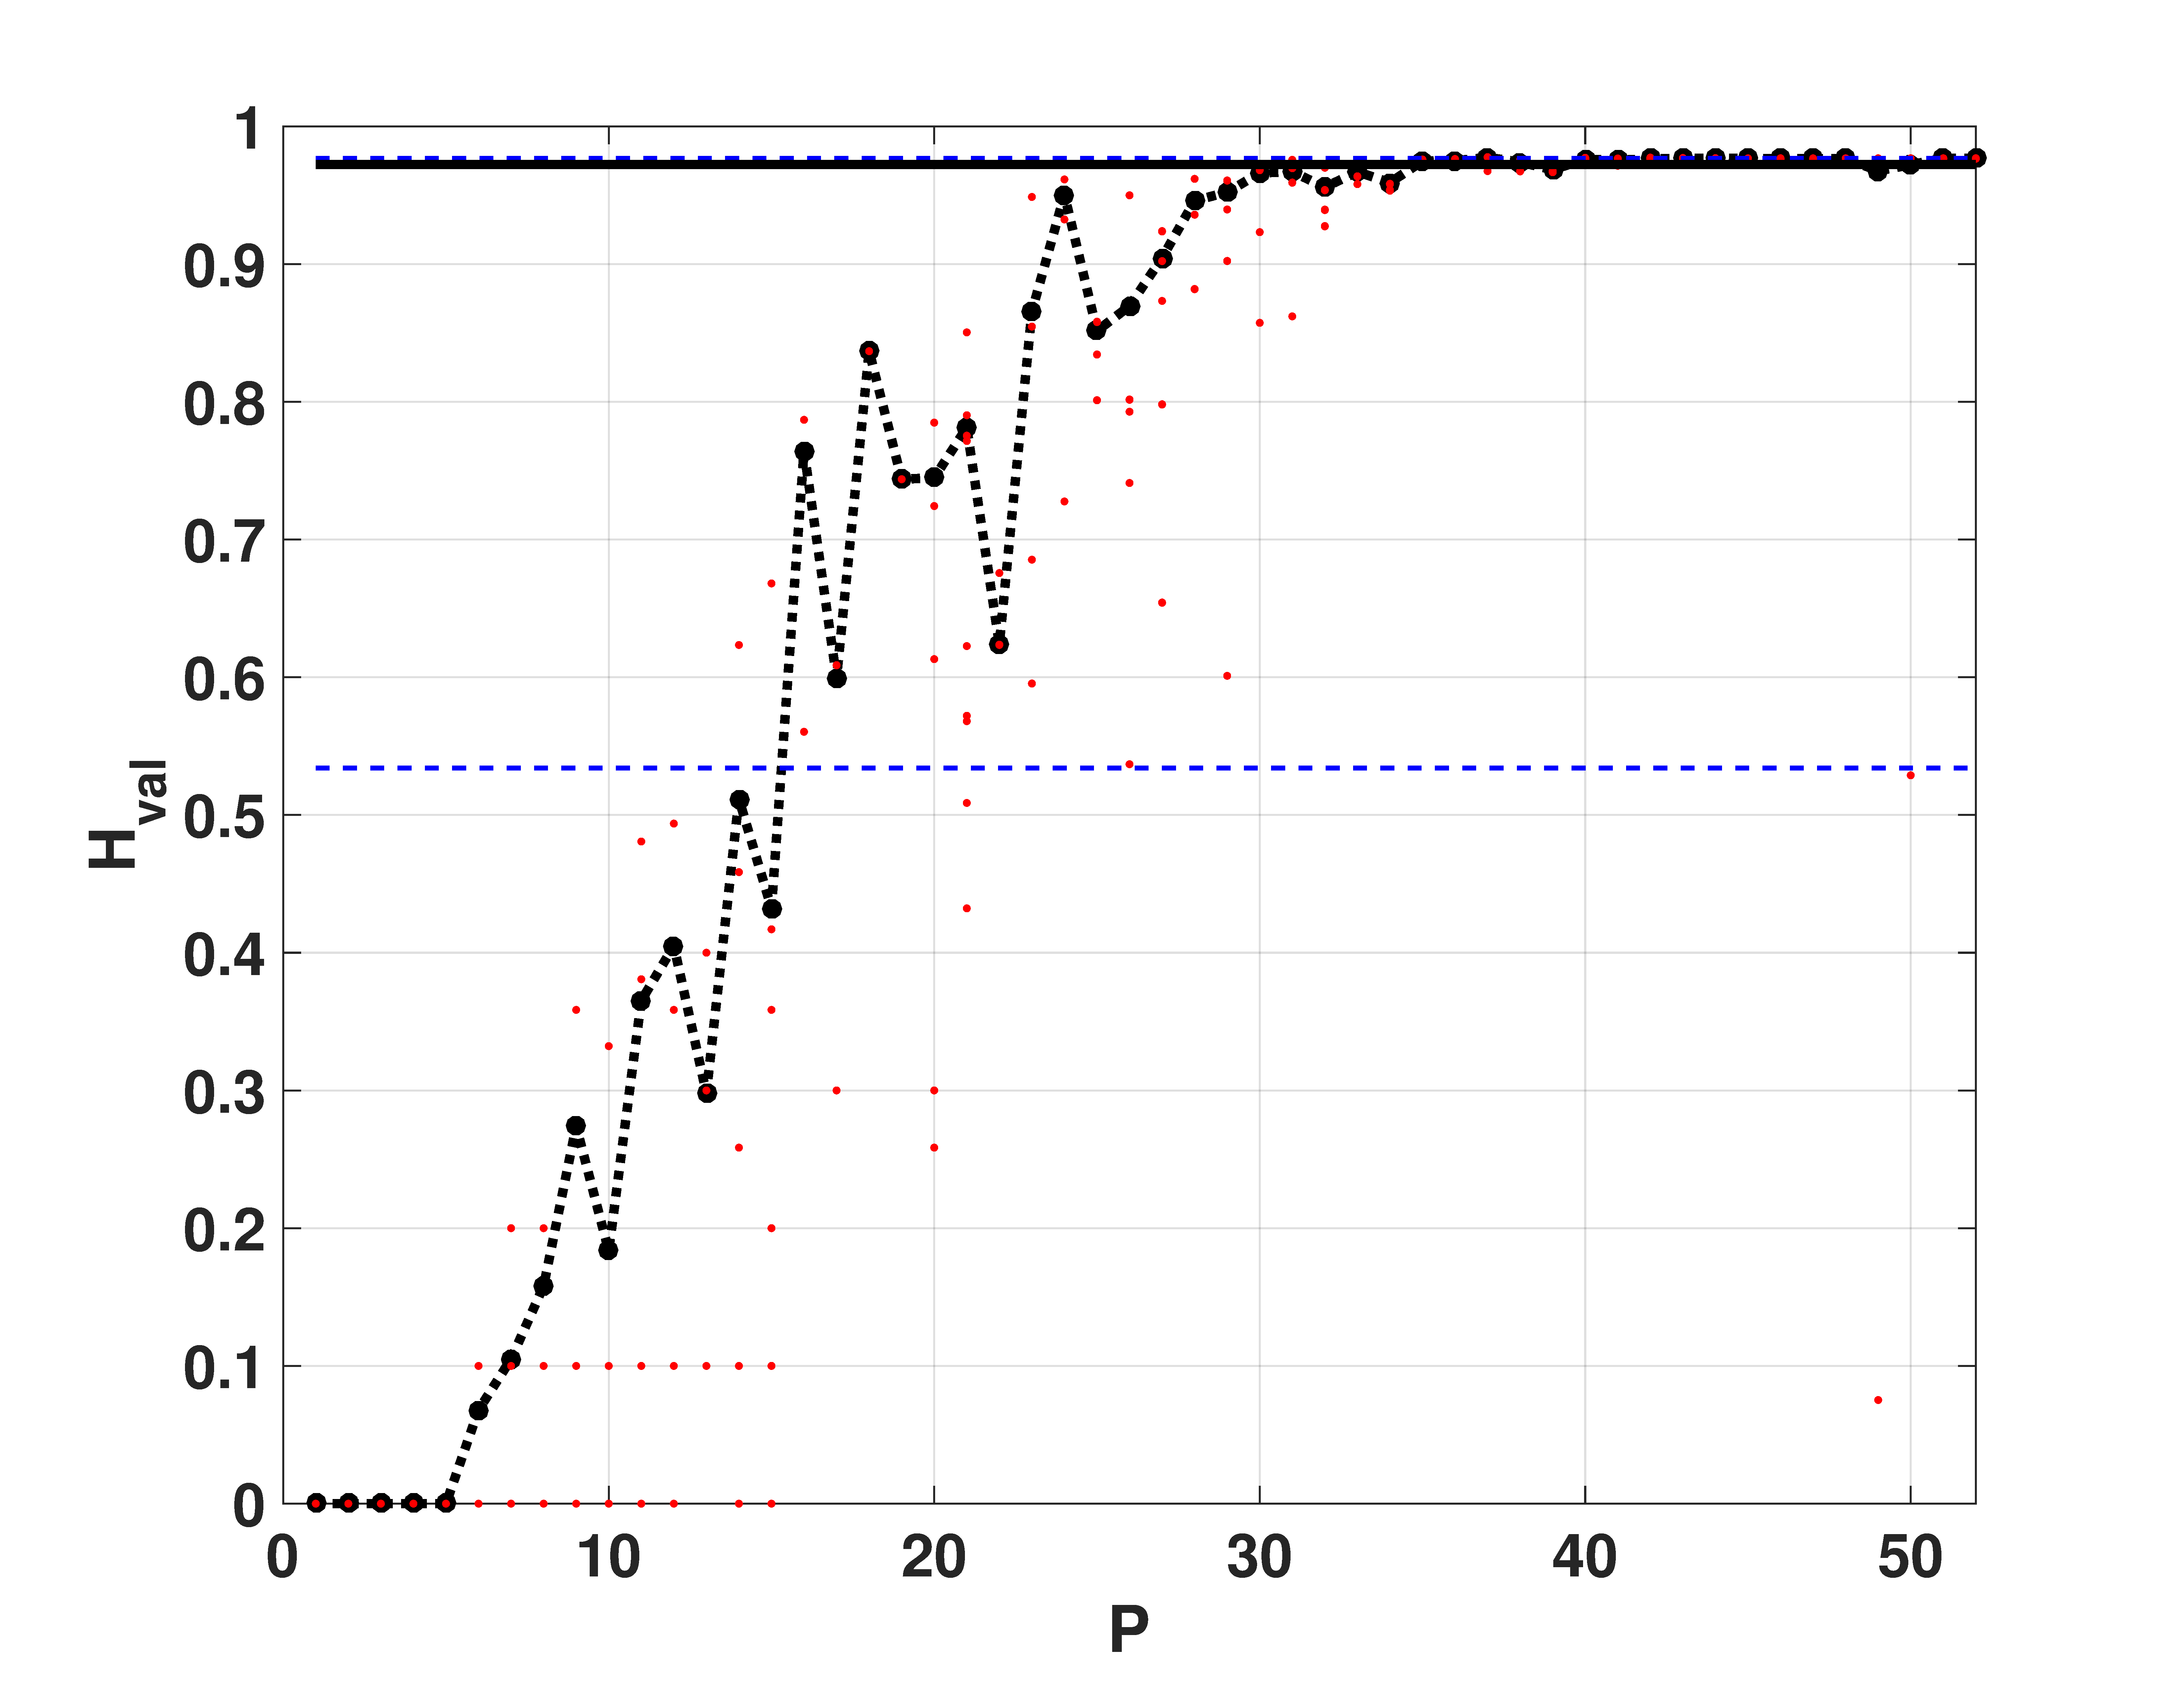
\includegraphics[width=.32\textwidth]{Hval_Switch}
	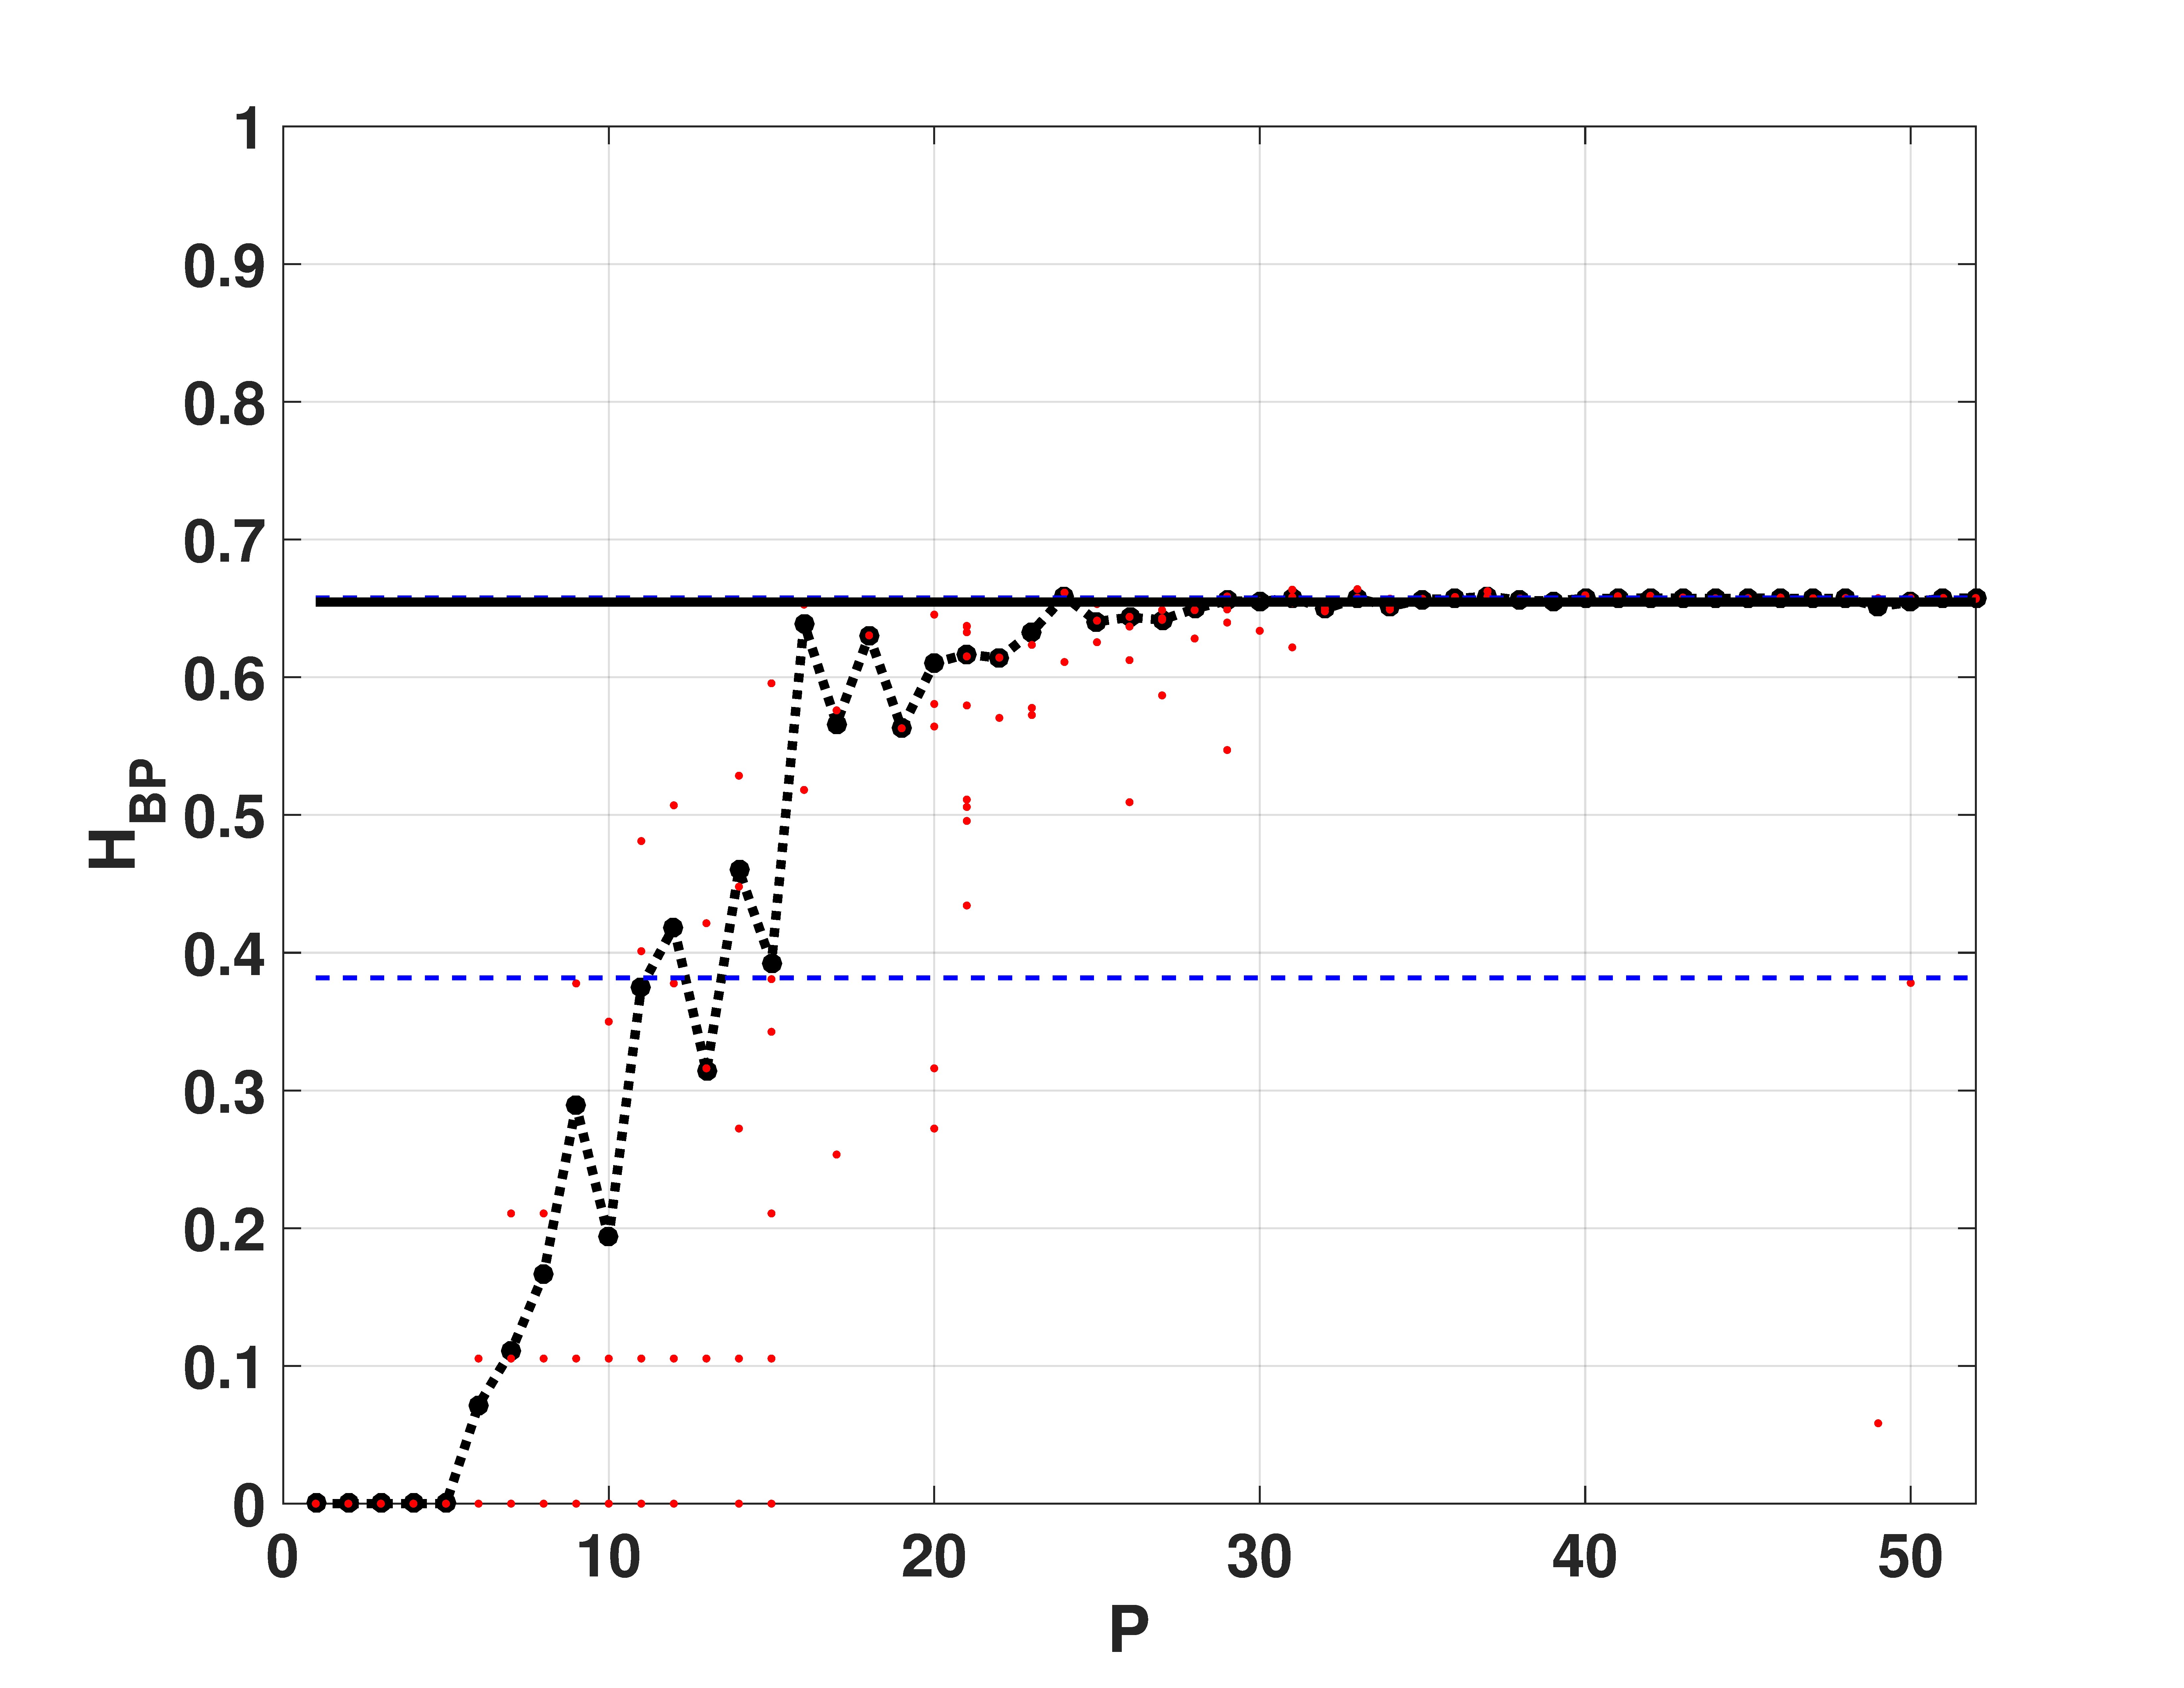
\includegraphics[width=.32\textwidth]{Hbp_Switch}
	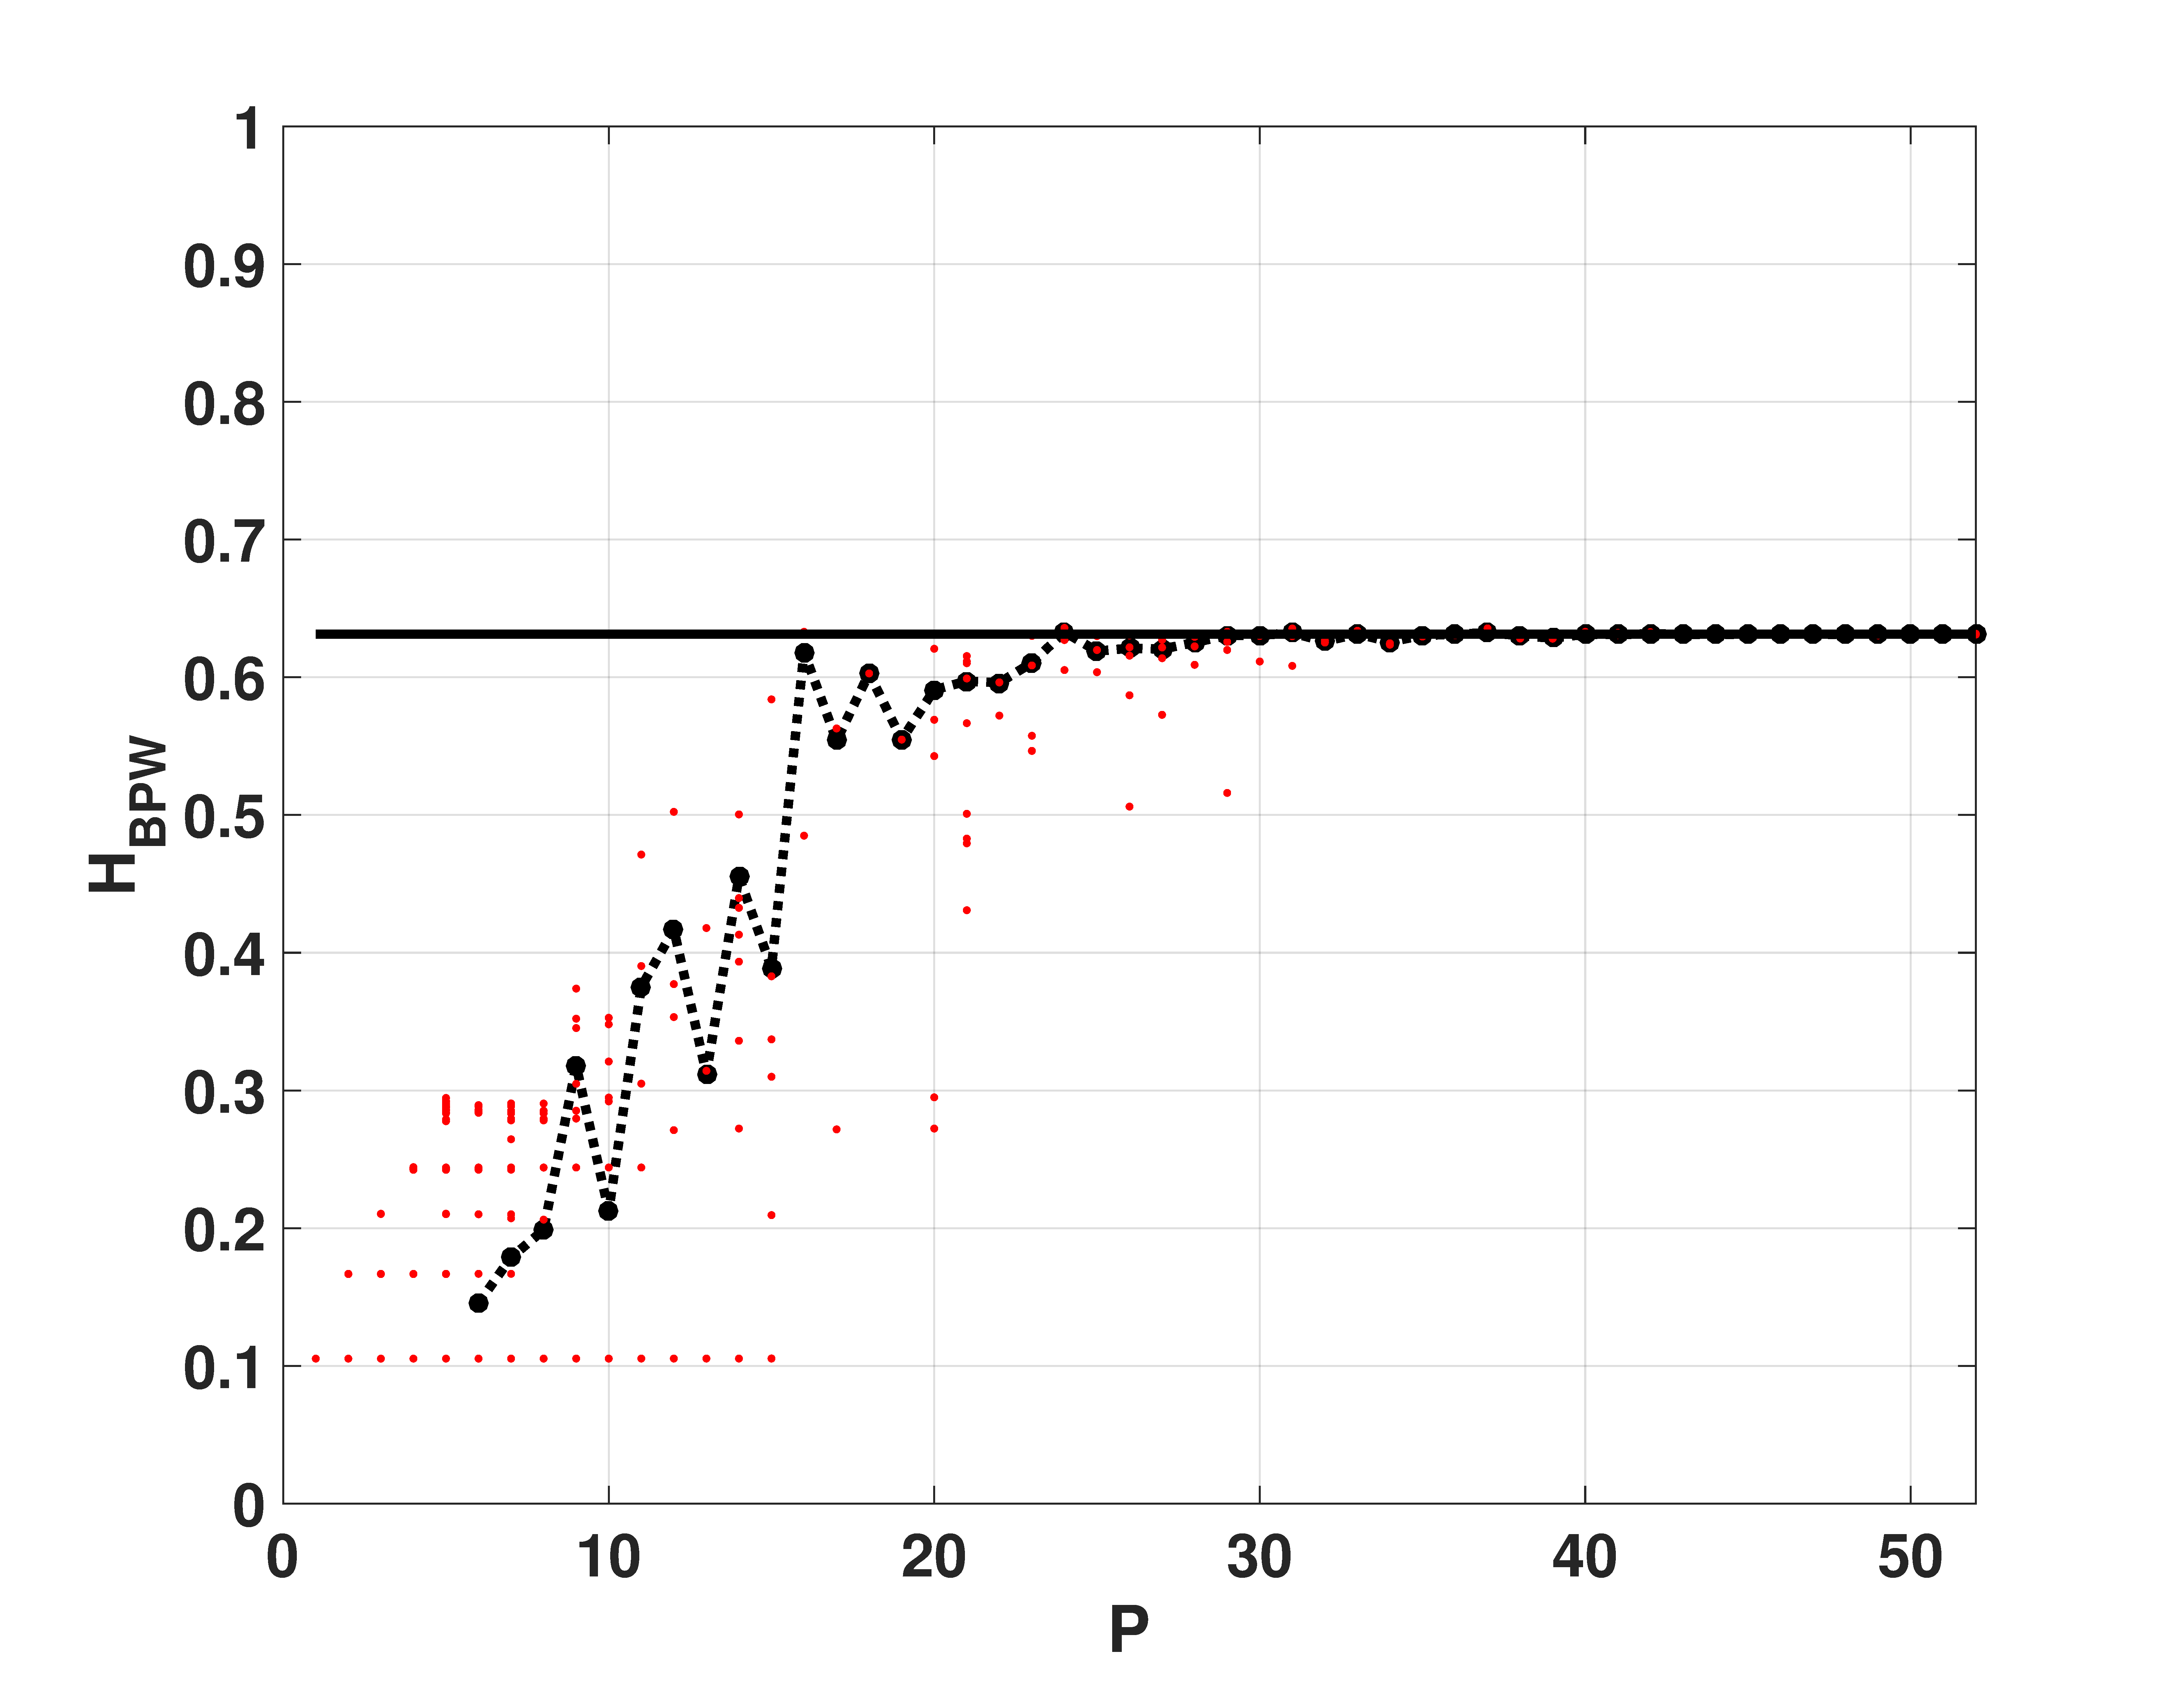
\includegraphics[width=.32\textwidth]{Hbpw_Switch}
	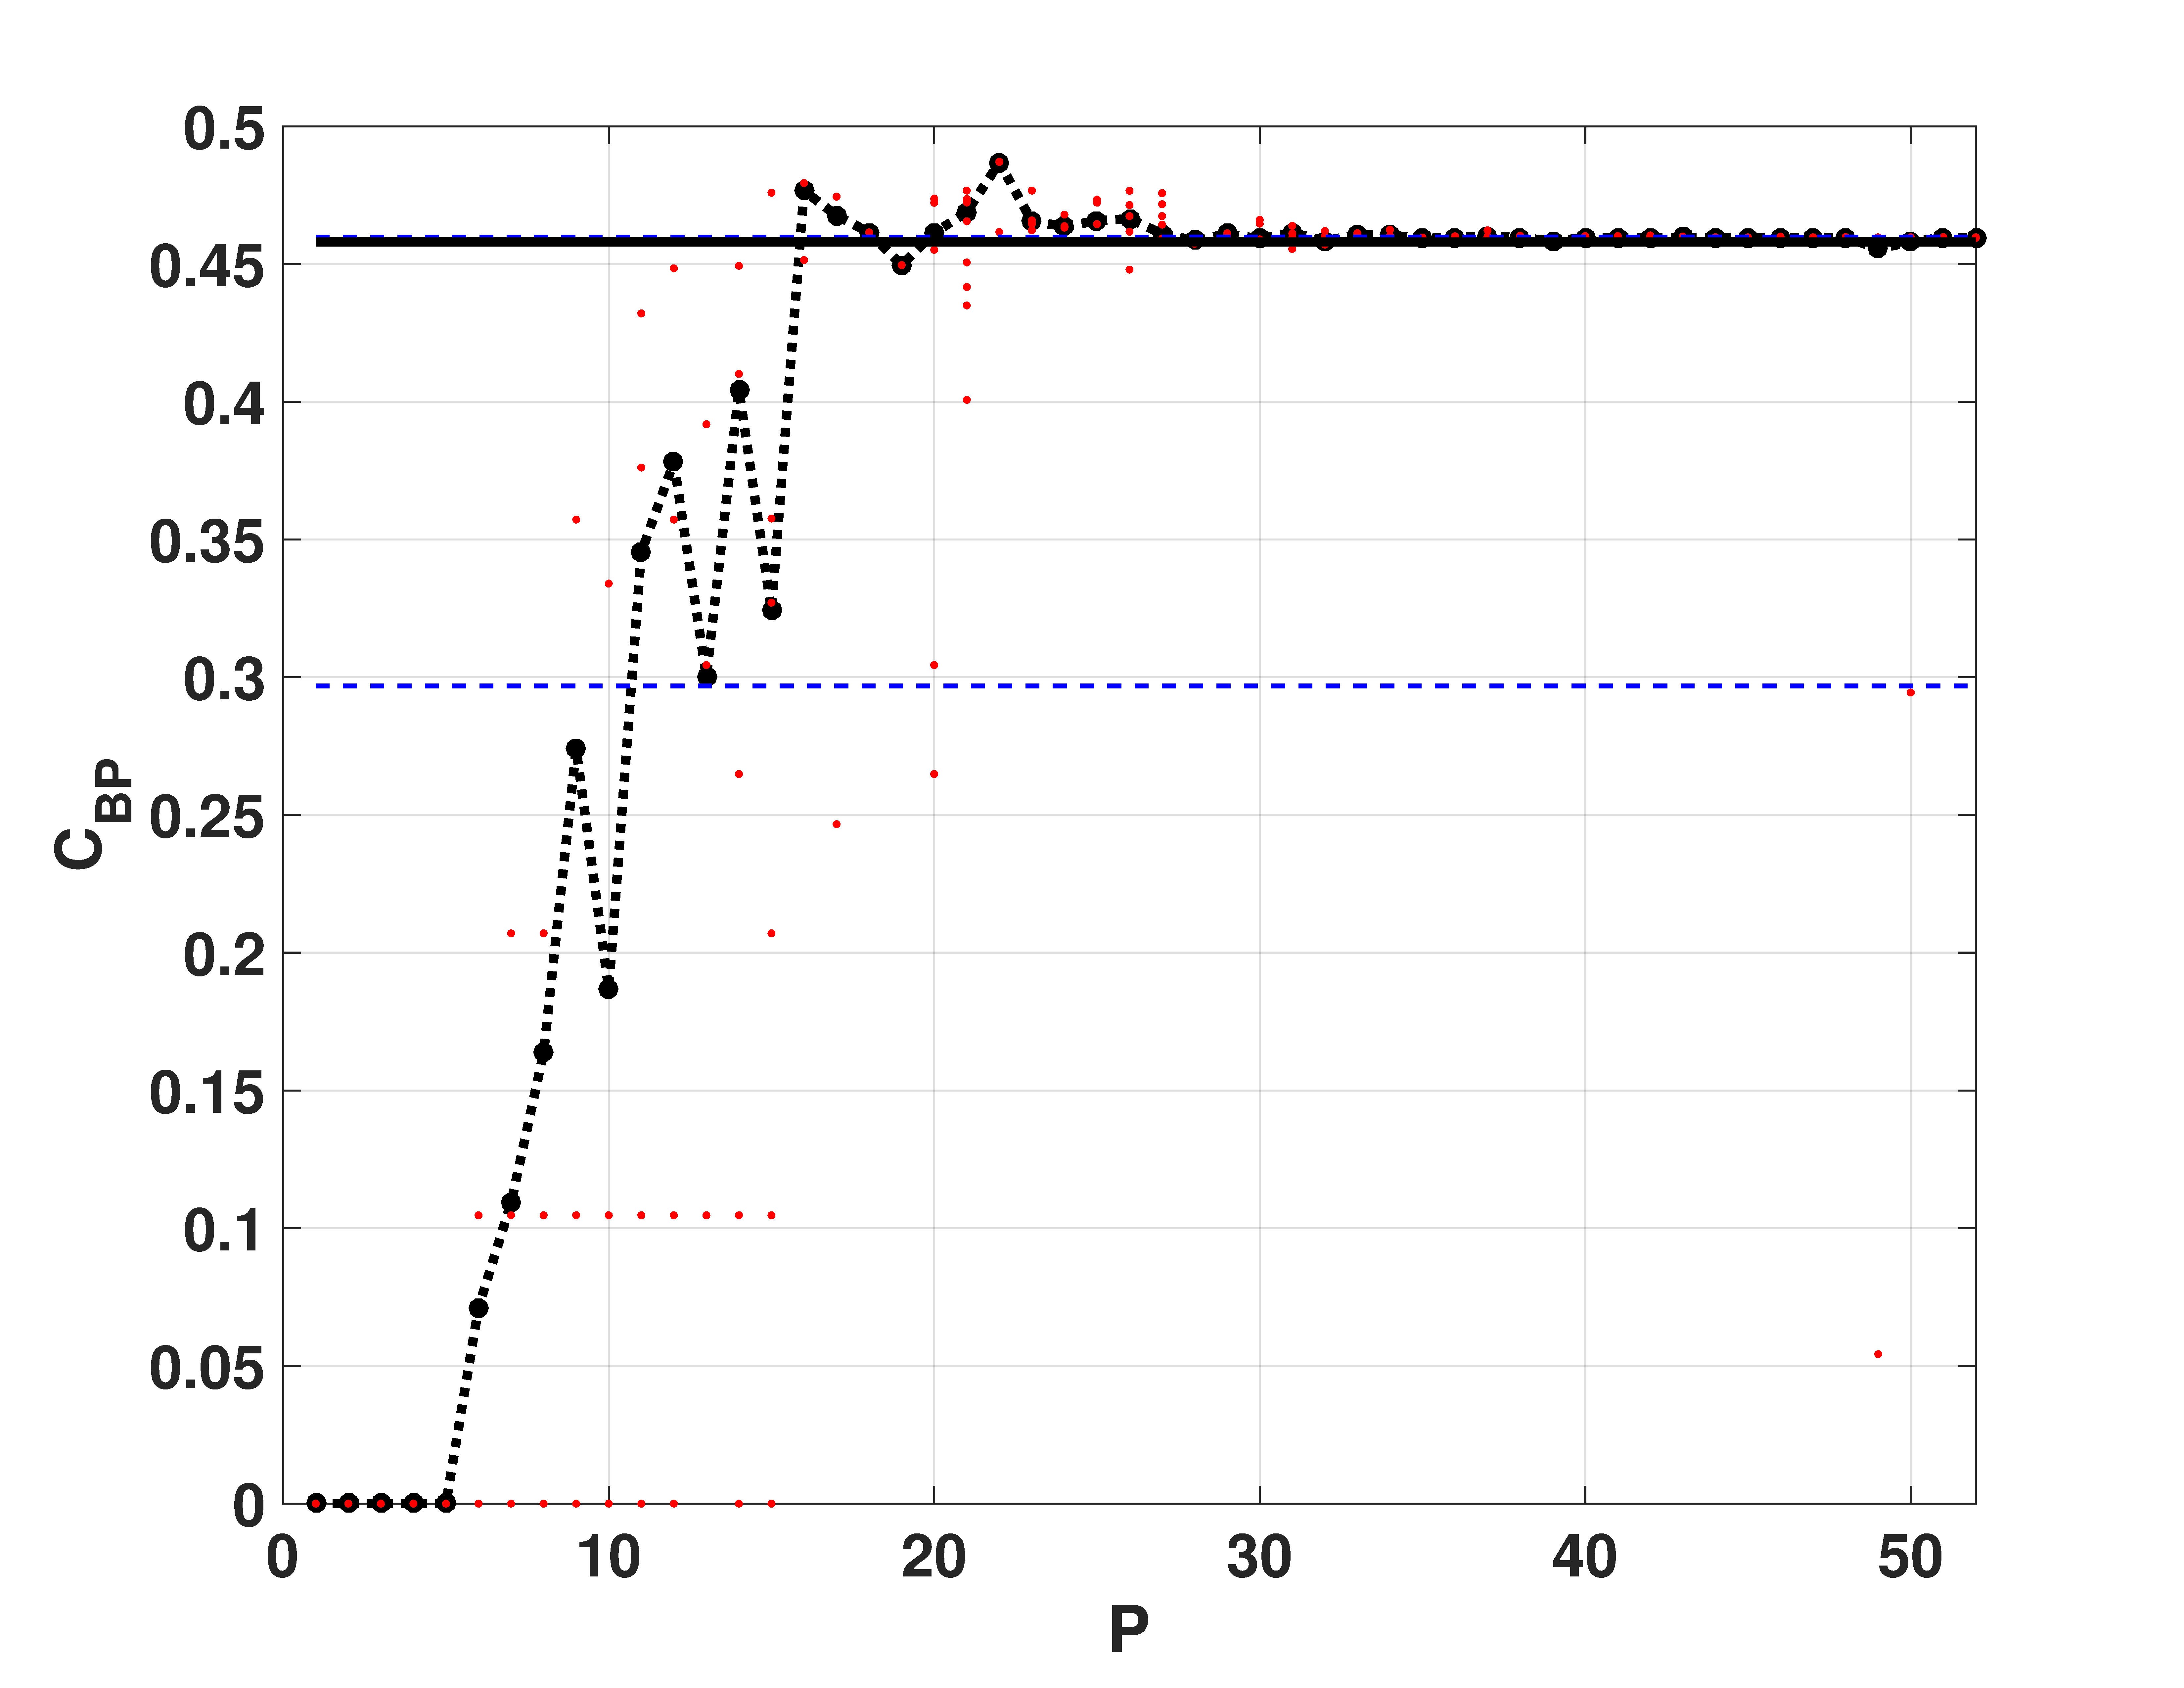
\includegraphics[width=.32\textwidth]{Cbp_Switch}
	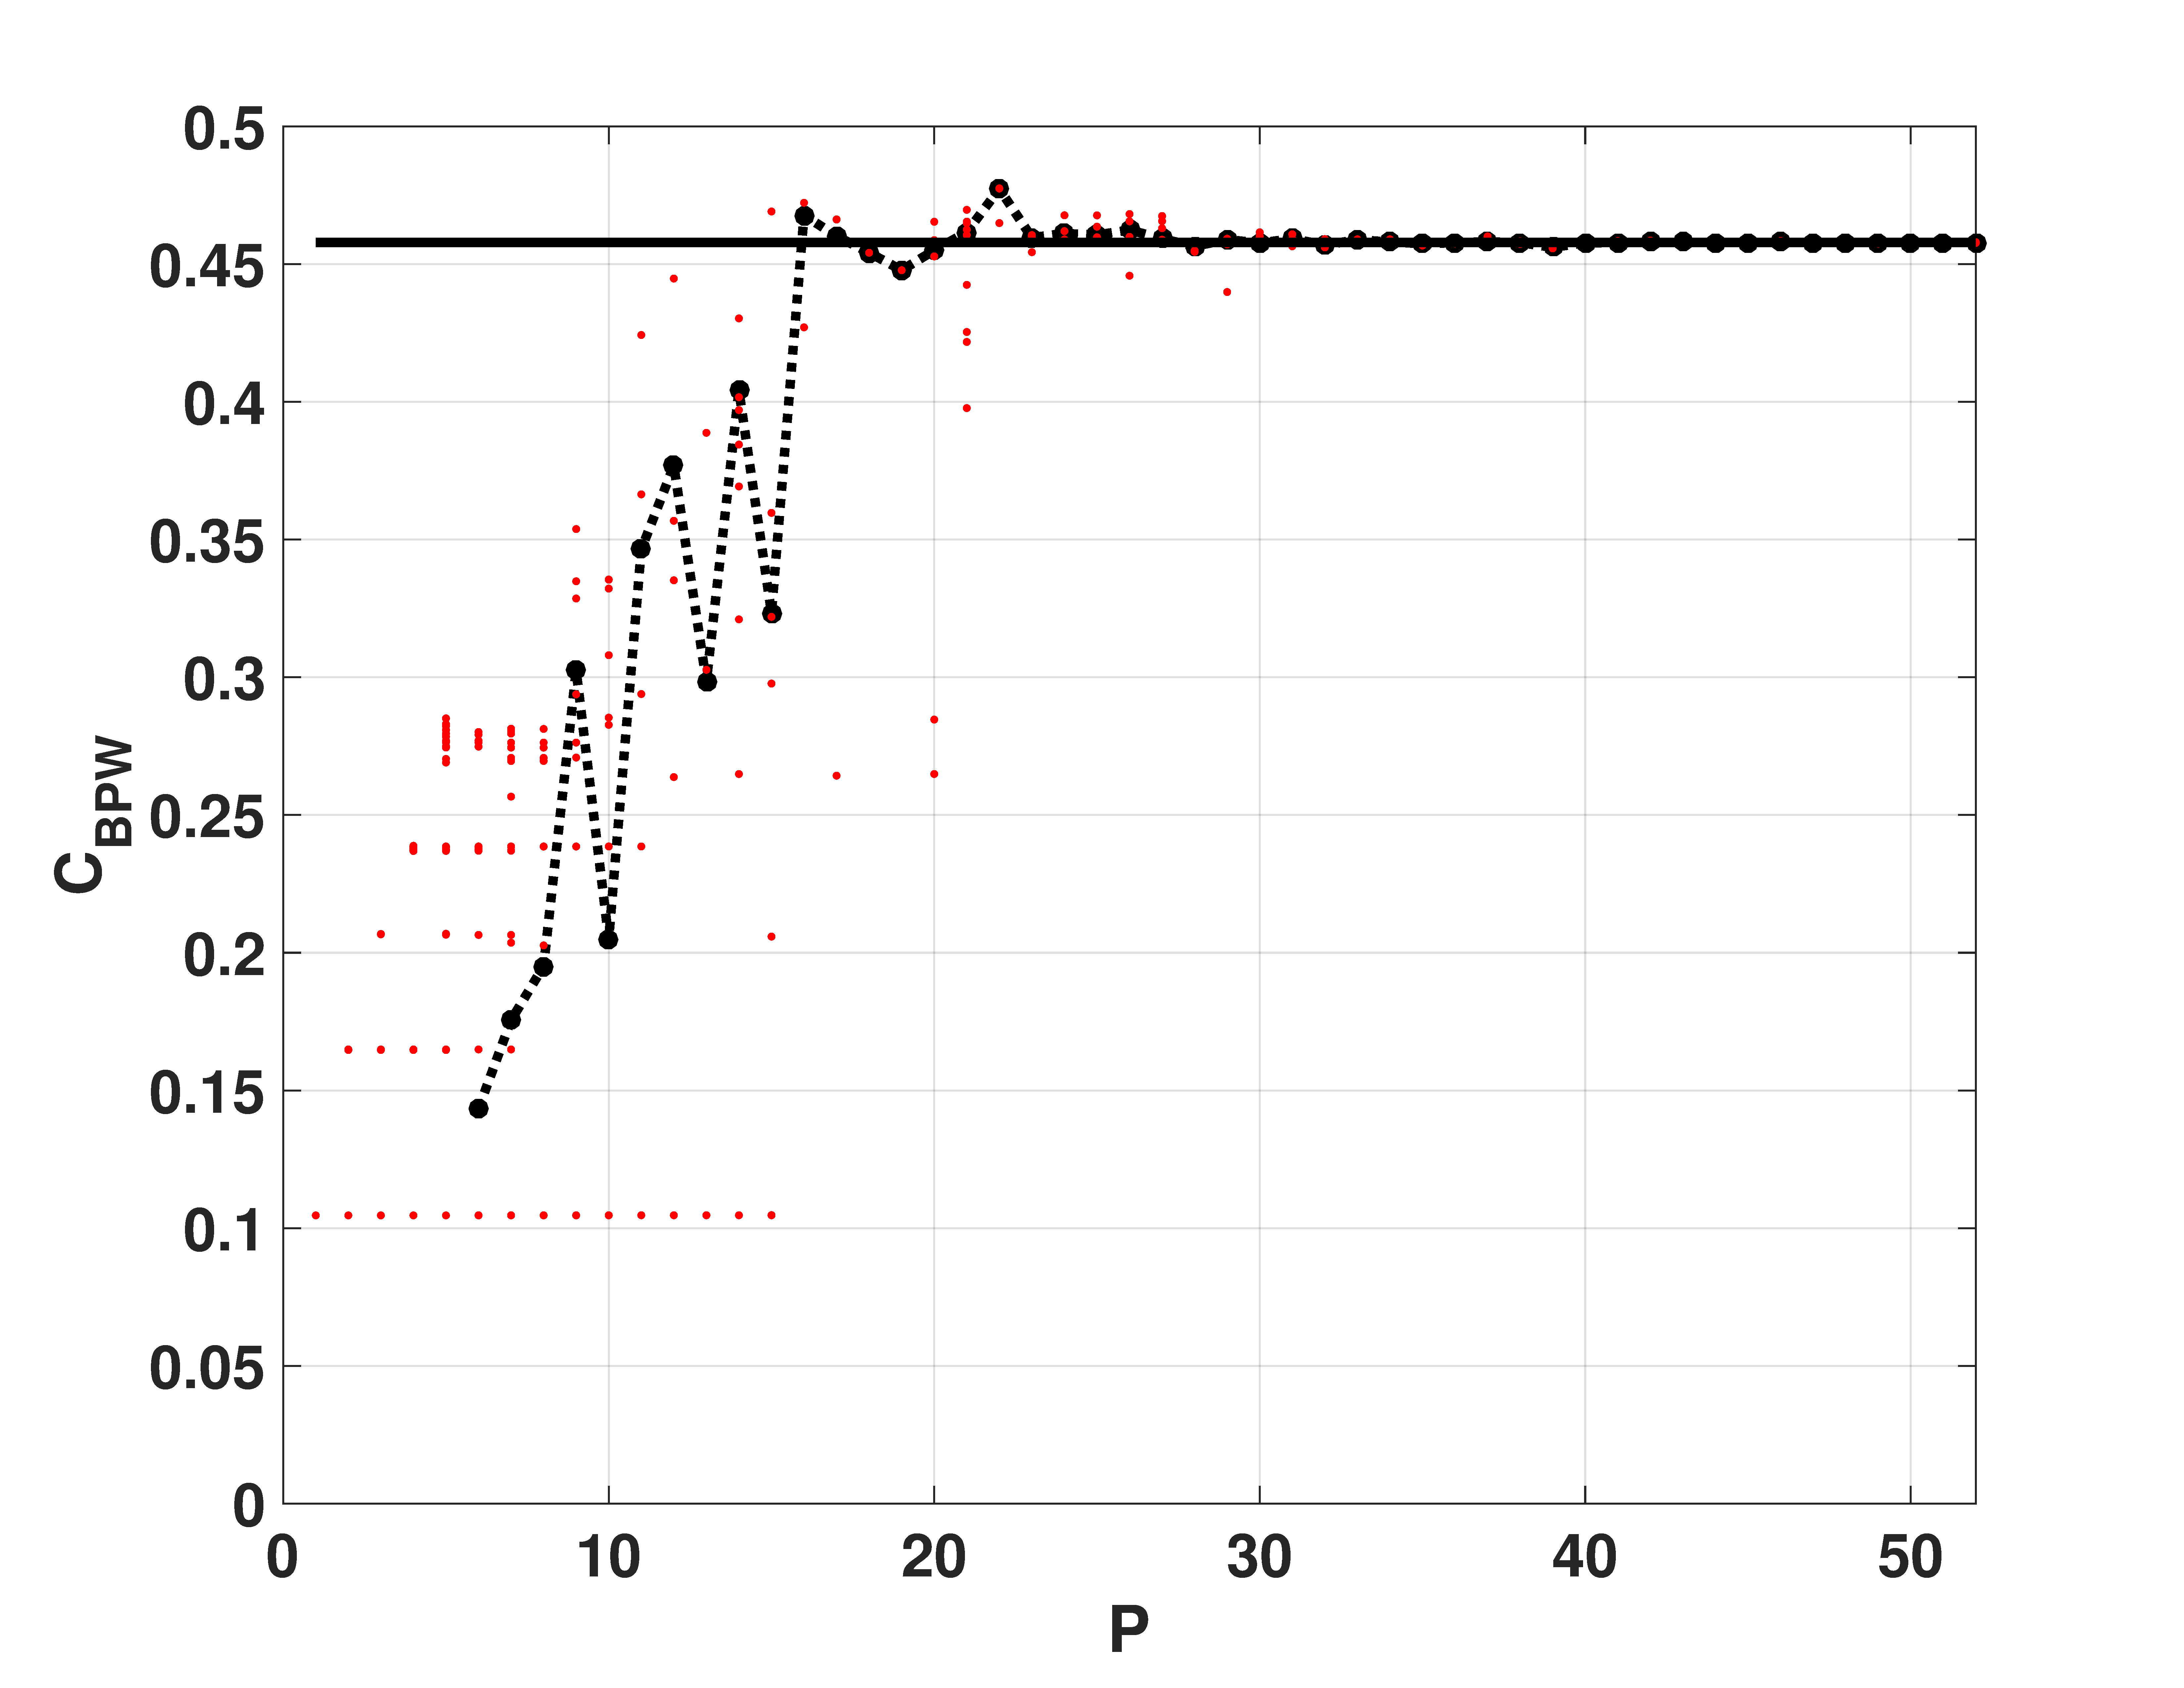
\includegraphics[width=.32\textwidth]{Cbpw_Switch}
	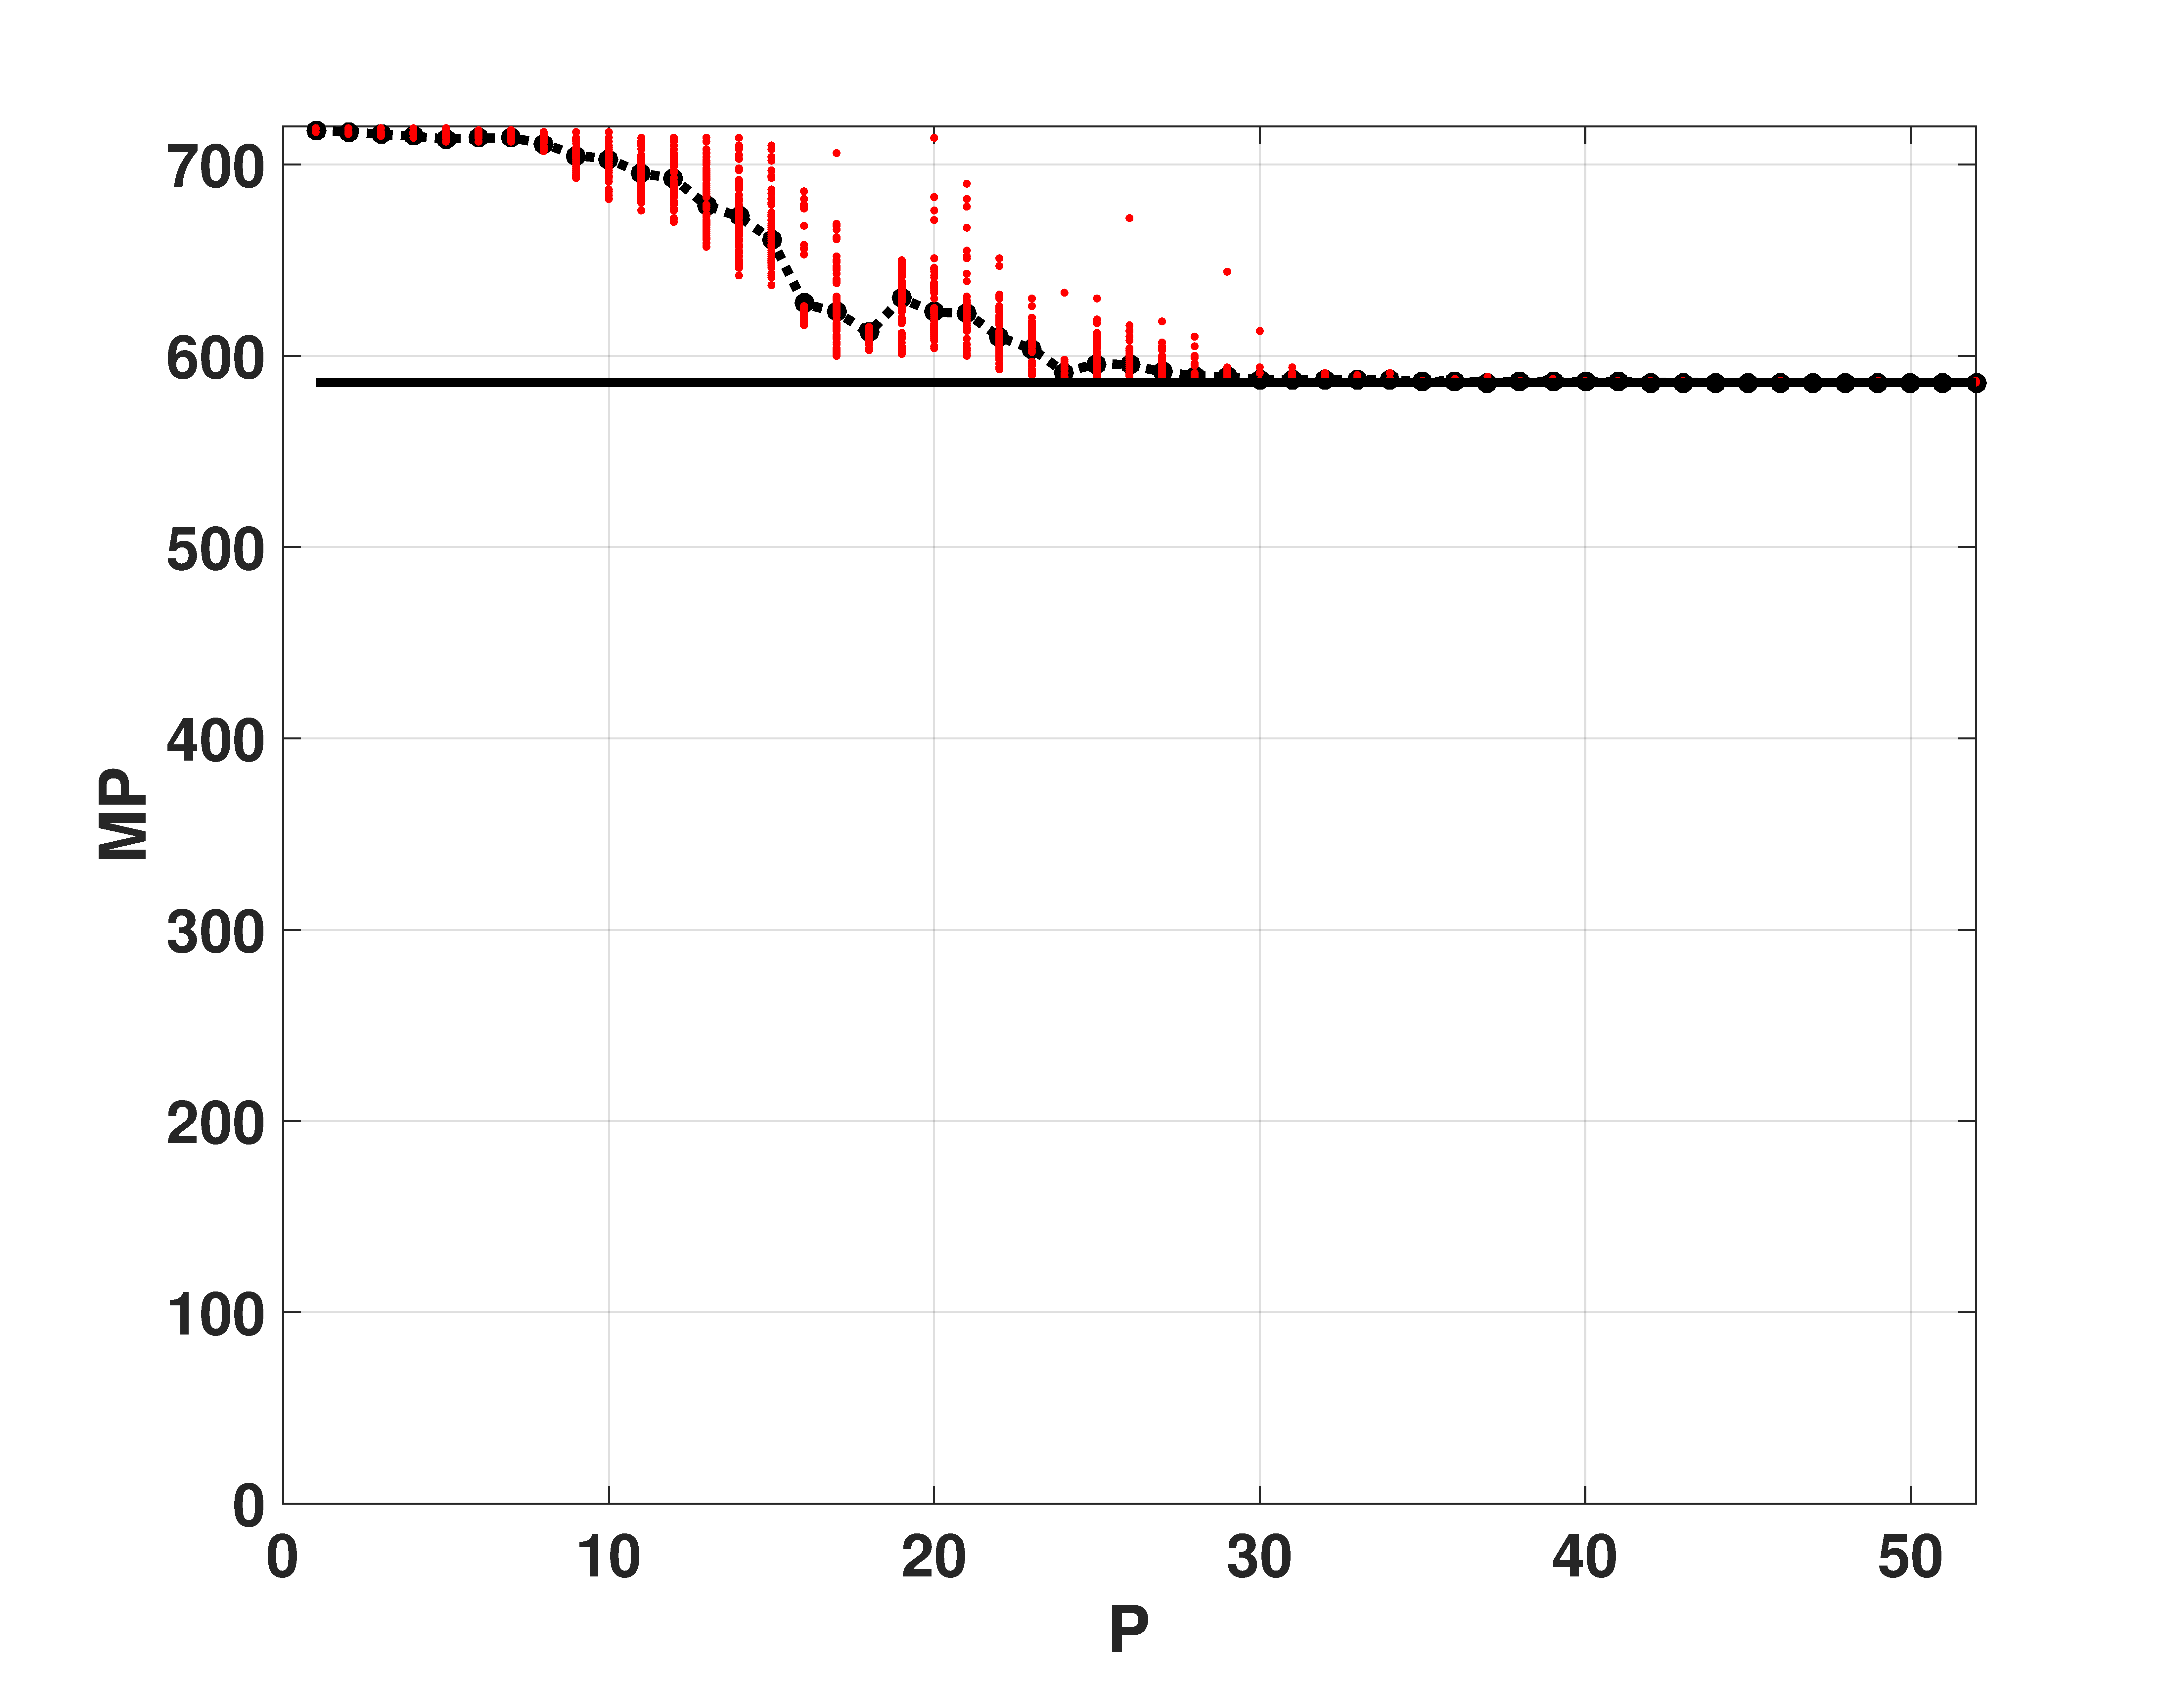
\includegraphics[width=.32\textwidth]{MP_Switch}
	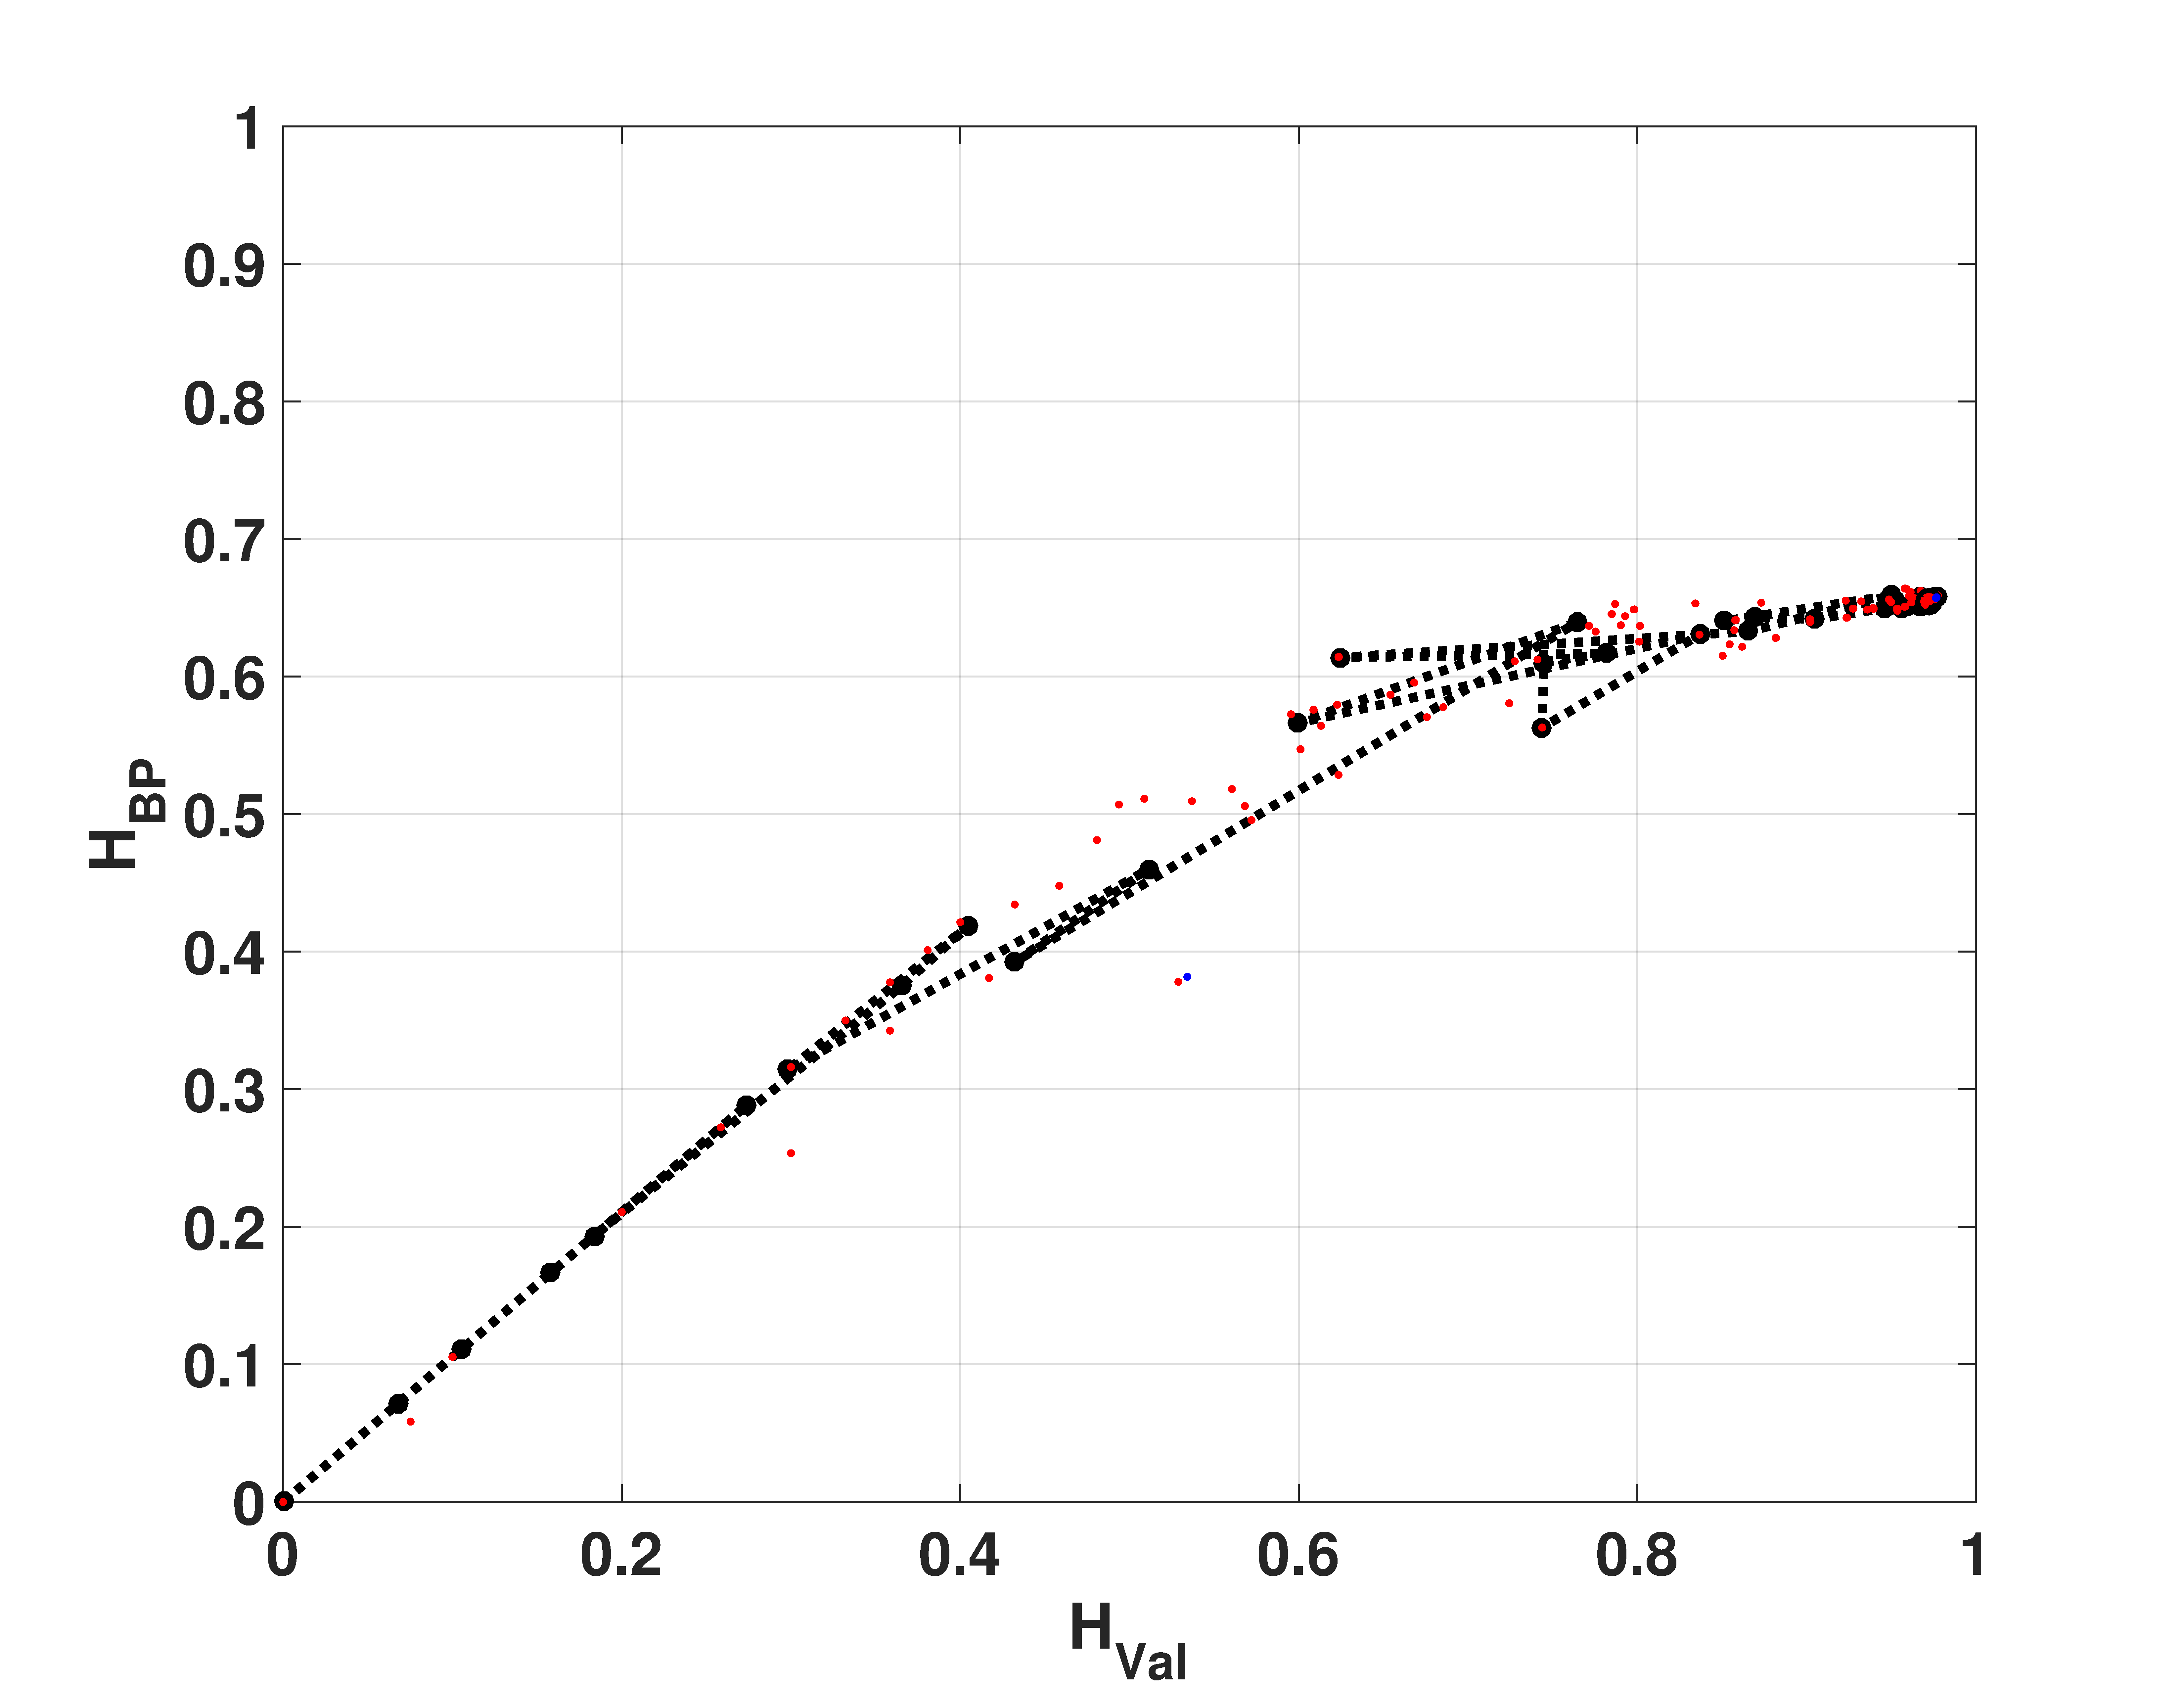
\includegraphics[width=.32\textwidth]{HbpHval_Switch}
	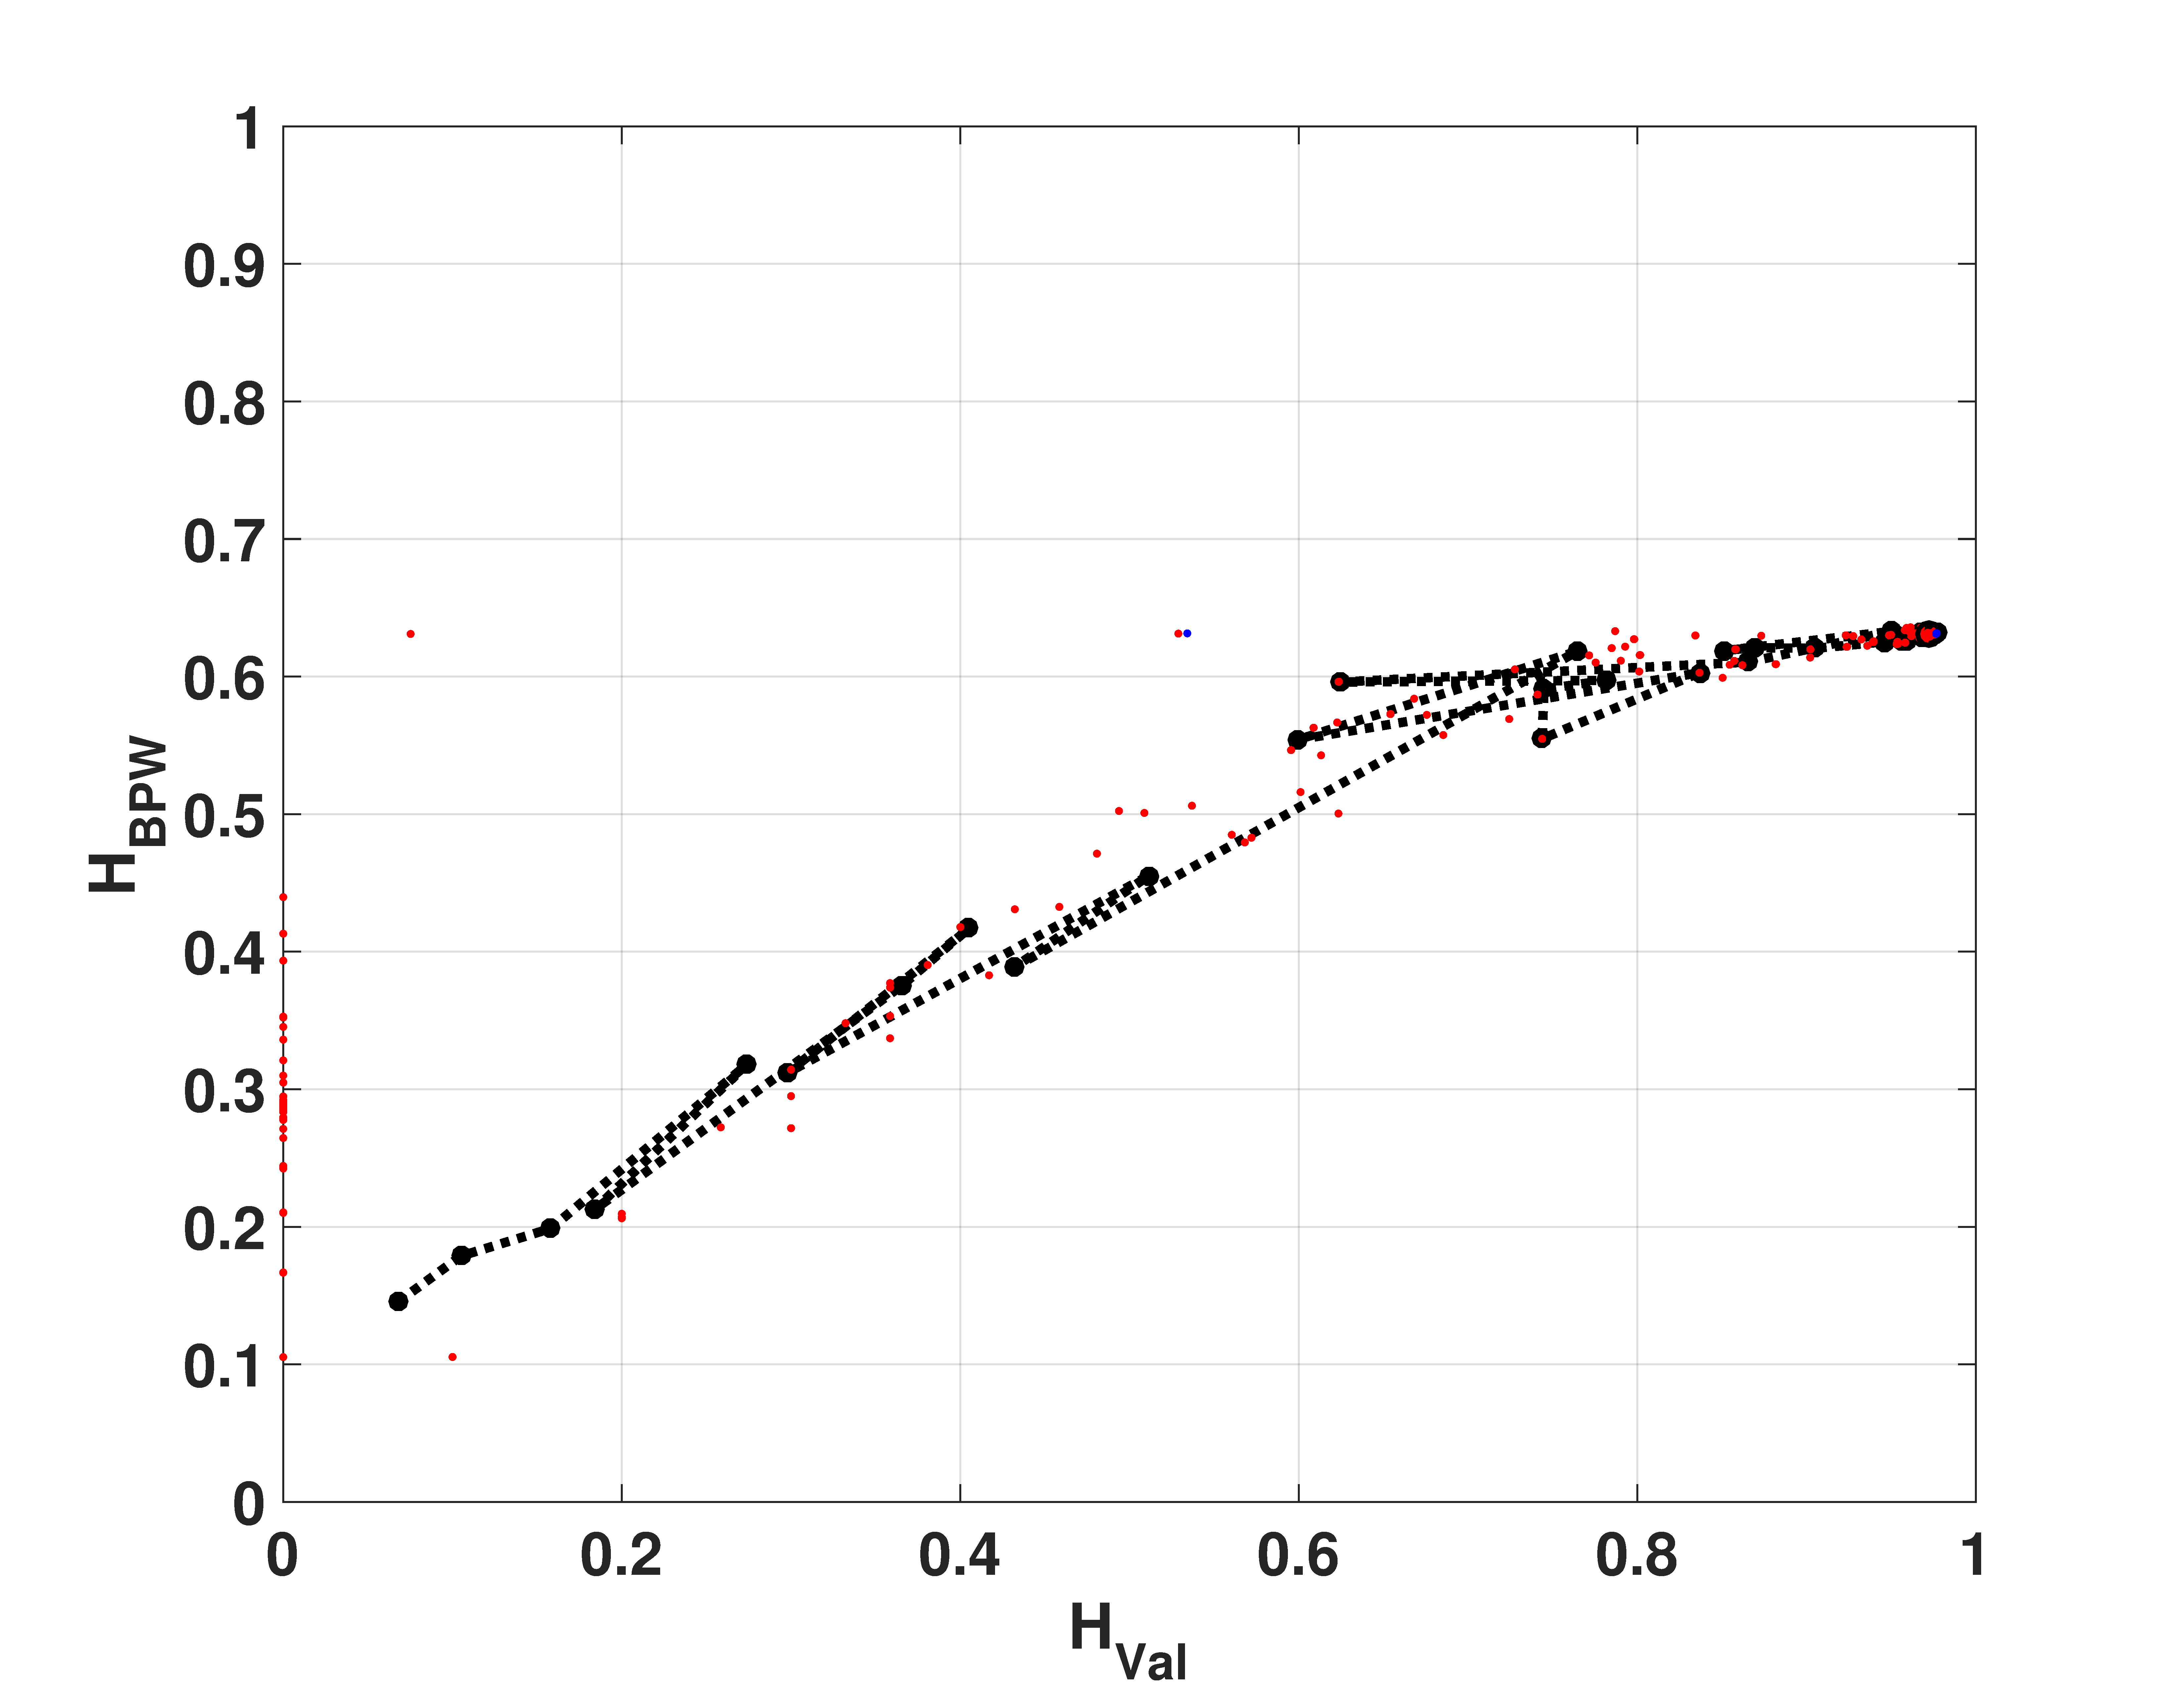
\includegraphics[width=.32\textwidth]{HbpwHval_Switch}
	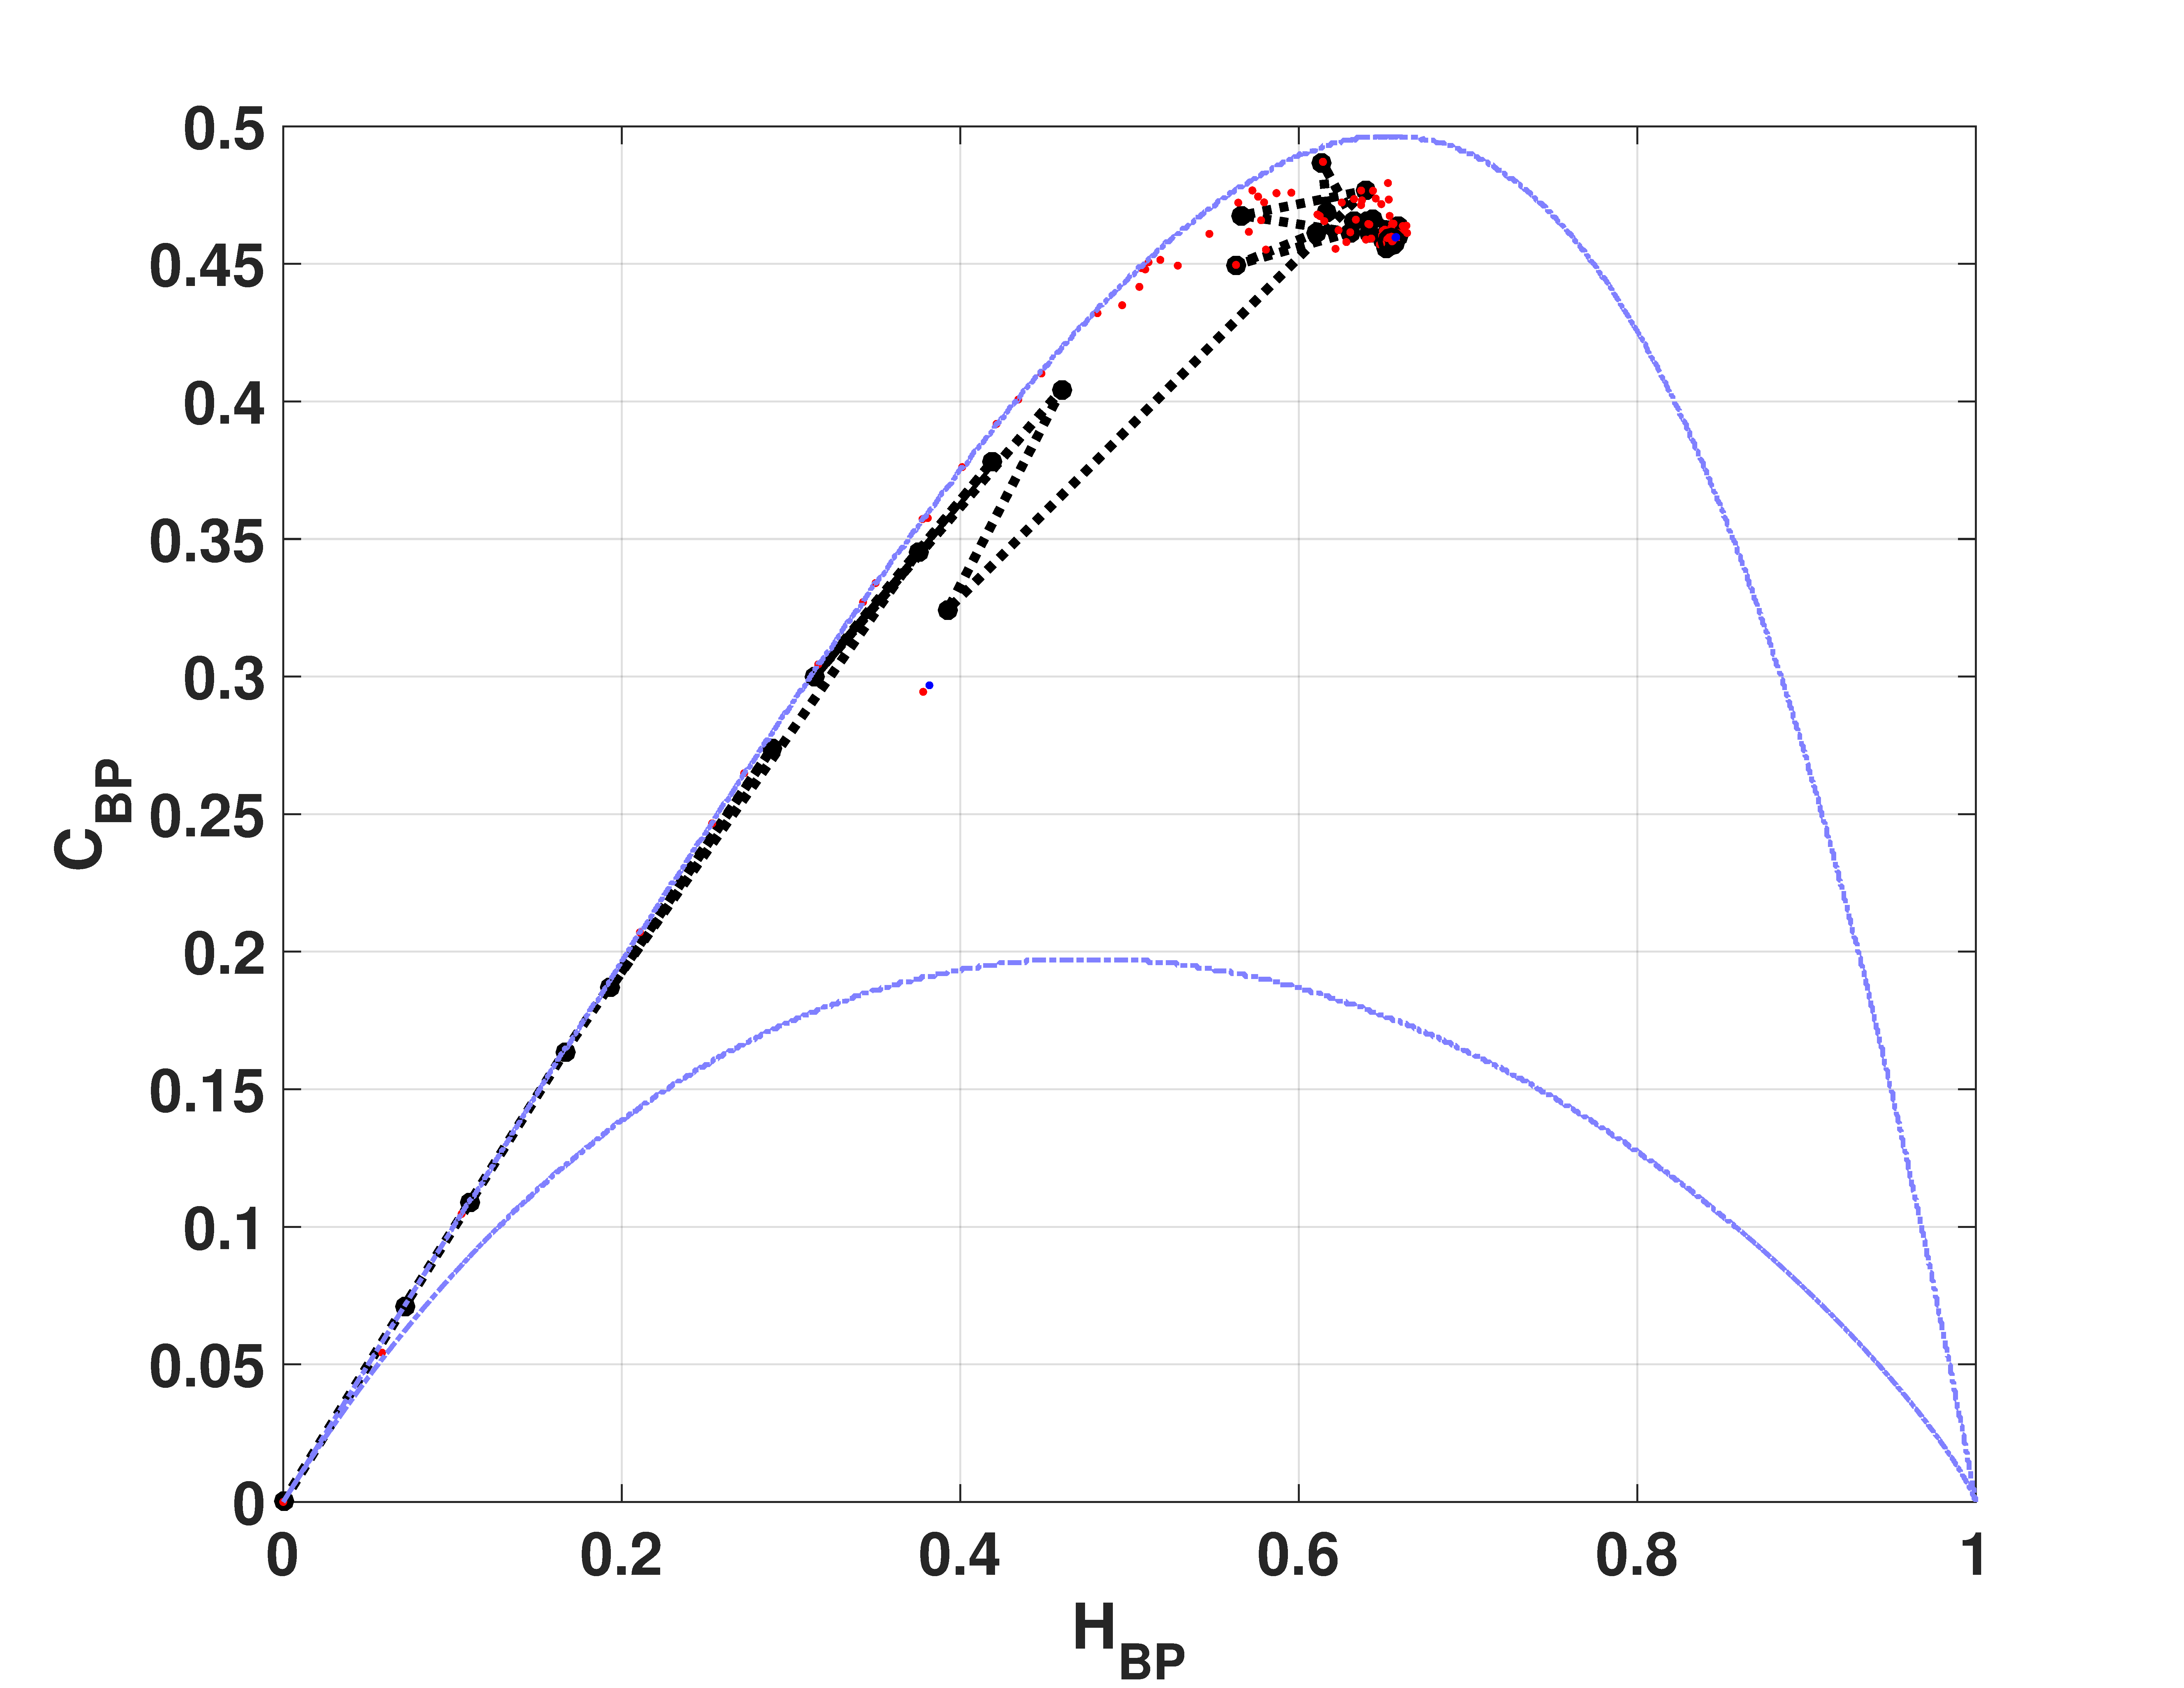
\includegraphics[width=.32\textwidth]{CbpHbp_Switch}
	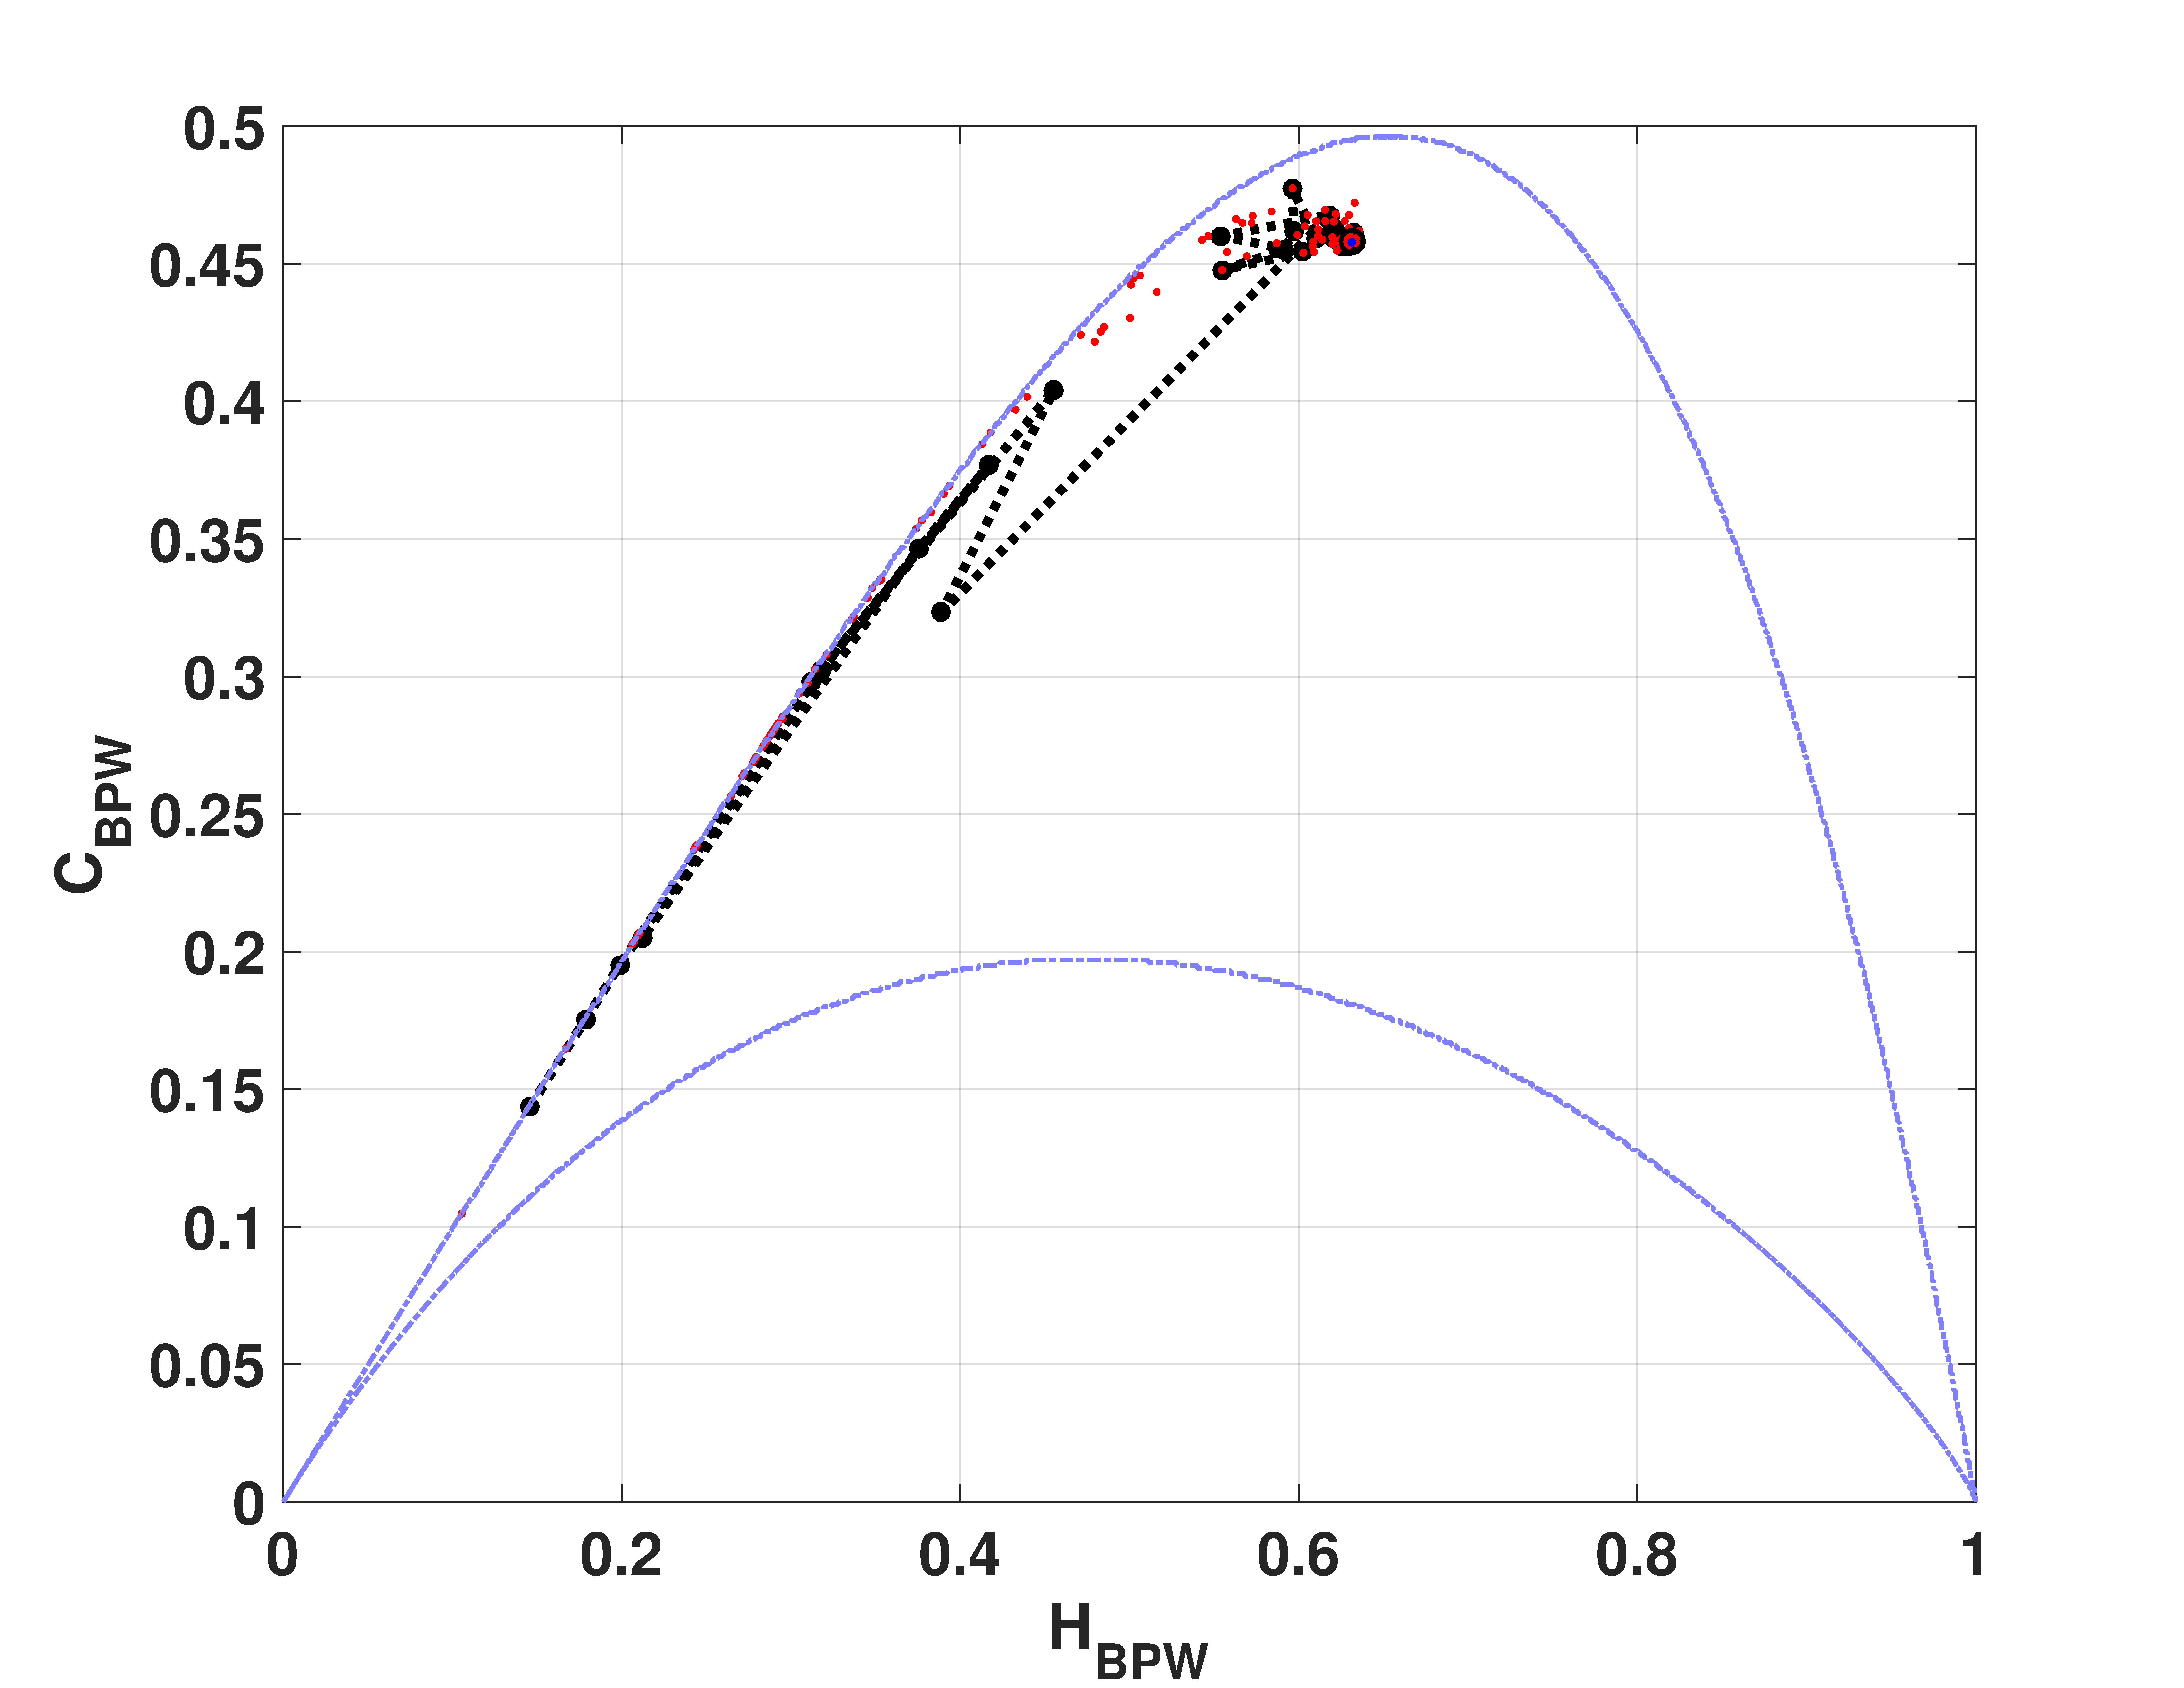
\includegraphics[width=.32\textwidth]{CbpwHbpw_Switch}
	\caption{Statistical properties of SWITCH,  using binary representation: (a) $H_{hist}$ vs $P$ (b) $H_{BP}$ vs $P$ (c) $C_{BP}$ vs $P$ (d) Number of missing ordering patterns $MP$ vs $P$. In Figures (a) to (d) dashed line correspond to floating point numbers. (e) representation in the $H_{hist},H_{BP}$ plane in the the binary numerical system.  The star represents the state for floating points numbers. (f) representation in the $H_{BP},C_{BP}$ plane.  The star represents the state for floating points numbers.  } \label{fig:seqbin}
\end{figure}